% -----------------------------------------------------------------------------------
% This template is brought to you by the                                            %
% Laboratory for Electrical Instrumentation and Embedded Systems                    %
% at the Albert-Ludwigs-Universität in Freiburg.                                    %
%                                                                                   %
% Please note: We do not provide technical support for this template.               %
% However, please feel free to contribute to this template on GitHub:               %
% https://github.com/emes-imtek/thesis_template                                     %
%                                                                                   %
% Authors: Alexander Richter, Till Steinmann, Andreas Reichenbach                   %
% -----------------------------------------------------------------------------------

%! TEX root = main.tex
% Document settings
\input{settings+/docclass}
% select chair
\input{settings+/selectchair}
% Supported chairs
% EMES
% SYSCOP
\selectchair{SYSCOP}
\input{settings+/settings}  % Custom variables are located in settings+/variables.tex

% Compile specific chapters only
\includeonly{
            % chapters/introduction,
            chapters/theory,
            chapters/proposed,
            %  chapters/benchmark,
            %  chapters/experiment,
            %  chapters/conclusion_outlook,
            %  chapters/acknowledgments,
             }

% -----------------------------------------------------------------------------------
% Information about the work and the author
% -----------------------------------------------------------------------------------
% Author
\author{Jingtao Xiong}
\matrikelnr{5986123}

% -----------------------------------------------------------------------------------
% English chair and thesis info
% -----------------------------------------------------------------------------------
\institute{IMTEK -- Department of Microsystems Engineering}
\ifchair{EMES}
    \chair{Laboratory for Electrical Instrumentation and Embedded Systems}\fi
\ifchair{SYSCOP}
    \chair{Systems Control and Optimization Laboratory}\fi

\thesisType{Master's Thesis}
\thesisTitle{Riccati-based Primal Regularizations in Interiror-Point Solvers for Indefinte Quadratic Programs}
\submitDate{March 10, 2022} % Use \today for the date of compilation
\editingTime{July 13, 2021 - March 10, 2022}

% Examiners
\firstExaminer{Prof. Dr. Moritz Diehl}
\firstExaminerDepartment{IMTEK -- Department of Microsystems Engineering}
\firstExaminerChair{Systems Control and Optimization Laboratory}

\secondExaminer{Prof. Dr. Max Doe}
\secondExaminerDepartment{IMTEK -- Department of Microsystems Engineering}
\secondExaminerChair{Laboratory for something that likely has a long title as well}

% Supervisor
\supervisor{M.Sc. Jonnathan Frey}
\supervisorDepartment{IMTEK -- Department of Microsystems Engineering}
\supervisorChair{Systems Control and Optimization Laboratory}

% -----------------------------------------------------------------------------------
% Main document
% -----------------------------------------------------------------------------------
\begin{document}
    % -------------------------------------------------------------------------------
    % Language settings
    % -------------------------------------------------------------------------------
    % The default language is English
    % \selectlanguage{ngerman}  % Toggle ON/OFF

    % Language-specific settings that change automatically
    \input{settings+/language}

    % -------------------------------------------------------------------------------
    % Cover page
    % -------------------------------------------------------------------------------
    \input{settings+/front_matter/covers/cover}                     \cleardoublepage

    % -------------------------------------------------------------------------------
    % Abstract, Zusammenfassung, ToC
    % Lists: Symbols, Acronyms, Figures, Tables, Codes
    % -------------------------------------------------------------------------------
    % Abstract in English and German
    \pagenumbering{Roman}  % I, II, III..
    \include{chapters/abstract}
    \include{chapters/zusammenfassung}

    % Table of contents
    \tableofcontents

    % List of Symbols & Acronyms
    \include{settings+/front_matter/lists&indexes/symbols}
    \include{settings+/front_matter/lists&indexes/acronyms}

    % List of Figures & Tables
    \include{settings+/front_matter/lists&indexes/figureindex}
    \include{settings+/front_matter/lists&indexes/tableindex}

    % List of C++,C,Python,... Code listings
    \include{settings+/front_matter/lists&indexes/codeindex}

    % -------------------------------------------------------------------------------
    % Main Content
    % -------------------------------------------------------------------------------
    % Introduction, Goals of the work, Fundamentals, State of the Art, Content,
    % Simulation, Real World Experiment, Outlook, Acknowledgements
    \cleardoublepage
    \pagenumbering{arabic}  % 1, 2, 3..

    % Use \include for main content. It automatically calls \clearpage.
    \documentclass[class=scrbook, crop=false]{standalone}
\usepackage[subpreambles=true]{standalone}
\ifstandalone
    \input{../settings+/settings}
\fi

% ----------------------------------------------------------------------------
%                                Introduction
% ----------------------------------------------------------------------------
\begin{document}

\chapter{Introduction}
\label{Chapter::Introduction}

\section{Motivation}
\label{sec:motivation}

In the field of optimal control, 
direct multiple shooting~\cite{bock1984multiple} is a widely used method for solving continuous-time optimal control problems,
which transcribes the OCP into a nonlinear programming problem by discretizing the time horizon into multiple shooting intervals~\cite{Diehl2018}.

This NLP is commonly solved by SQP, which computes each step from a QP subproblem 
which inherits an optimal control structure that Riccati recursion can exploit \cite{rao1998application}.
To retain the fast local convergence of SQP, 
the QP subproblems are often formulated with the exact Hessian of the Lagrangian \cite{BoggsTolle1995},
this could result in an indefinite Hessian thus a nonconvex QP as subproblem, 
which is not guaranteed to have a unique solution and can cause the Riccati recursion to fail.

A common remedy is to regularize at the SQP level,
i.e.\ to modify the QP Hessian before the QP is passed to the solver.
Such a correction is decided from the Hessian of the QP subproblem alone and therefore overlooks two aspects.
First, inside an interior point method, the barrier term of the inequality constraints adds curvature to the Hessian,
which can render the system well-defined even when the QP Hessian itself is indefinite.
Second, when the correction targets the full Hessian, it ignores that positive definiteness of the reduced Hessian
is already sufficient for the QP to have a unique solution.

This thesis therefore regularizes at the QP level, inside the solver,
where the correction is computed from the factorized matrices and applied only when indefiniteness is actually detected.

\section{Contributions}
\label{sec:contributions}
The main contributions of this thesis are the following:
\begin{enumerate}
    \item \textbf{Riccati-based primal regularization}, which regularizes the reduced Hessian blocks
    obtained from the Riccati recursion, only at the stages where the Cholesky factorization fails
    (Section~\ref{sec:riccati_primal_reg}).

    \item \textbf{An improved stage regularization strategy}, derived from showing that minimum perturbation
    propagates negative curvature through the cost-to-go matrix to the preceding stages
    (Section~\ref{sec:fail_minimal_perturbation}).

    \item \textbf{A proof of asymptotic inactivity}, so that the local convergence rate of the interior point method is preserved
    (Section~\ref{sec:asymptotic_inactivity}).

    \item \textbf{A benchmark of $175$ indefinite OCP QPs} collected from the SQP iterations of eight OCPs,
    with an analysis of where the indefiniteness originates (Chapter~\ref{Chapter::Benchmark}).

    \item \textbf{A numerical comparison} on this benchmark, in which the best Riccati-based method leaves $4$ instances unsolved,
    against $32$ to $59$ for full Hessian regularization and $15$ for inertia correction
    (Section~\ref{sec:comparison}).
\end{enumerate}

\section{Related Solvers}
\label{sec:related_solvers}
This thesis builds on two open-source software packages for embedded optimal control, \texttt{acados} and HPIPM.

\texttt{acados}~\cite{verschueren2020acadosmodularopensourceframework} is a modular framework for fast NMPC.
It transcribes the OCP by direct multiple shooting, solves the resulting NLP by SQP or its real-time iteration variant,
and passes the QP subproblems to one of several interfaced QP solvers.
When the exact Hessian is used, \texttt{acados} handles indefiniteness at the SQP level:
the QP Hessian can be regularized before the QP is passed to the solver or be replaced by a Gauss--Newton approximation.
In this thesis, \texttt{acados} is used to generate the SQP iterates from which the benchmark QPs are collected (Section~\ref{sec:benchmark_construction}).

HPIPM~\cite{frison2020hpipmhighperformancequadraticprogramming} is a primal--dual interior point solver
for OCP-structured QPs and the default QP solver in \texttt{acados}.
It solves the KKT system of each iteration by Riccati recursion, with a cost linear in the horizon length,
and relies on high-performance linear algebra routines tailored to the small and medium-sized matrices of optimal control.
HPIPM assumes a convex QP: the Riccati recursion requires the reduced Hessian blocks to be positive definite, so it fails on indefinite QPs.
This failure is precisely the criterion by which the benchmark QPs are collected (Section~\ref{sec:benchmark_construction}),
and the prototype solver used in the experiments reproduces the iteration behavior of HPIPM on convex QPs, 
so that the regularization is the only difference between the two (Section~\ref{sec:prototype}).


\section{Outline}
\label{sec:outline}
The remainder of this thesis is organized as follows.
Chapter~\ref{Chapter::Theoretical_Background} introduces the primal--dual interior point method for OCP-structured QPs,
the Riccati recursion used to solve its KKT system,
and the barrier update and step size control strategies adopted in the solver.
Chapter~\ref{Chapter::Primal_Regularization} classifies primal regularization by its target matrix,
develops the Riccati-based primal regularization,
derives the improved stage regularization strategy from the failure of minimum perturbation,
and proves that the regularization is asymptotically inactive.
Chapter~\ref{Chapter::Benchmark} constructs the benchmark of indefinite QPs from the SQP iterations of eight OCPs
and analyzes how the indefiniteness is distributed over the stages and where it originates.
Chapter~\ref{Chapter::Experiments} describes the prototype solver and the experiment setup,
compares the Riccati-based methods with full Hessian regularization and inertia correction on the benchmark,
and discusses the instances on which the methods fail.
Finally, Chapter~\ref{Chapter::Conclusion} summarizes the results and outlines directions for future work.

% You can use this to add content for standalone documents if you like
% In this case, we would like to show the acronyms and references.
\ifstandalone
    \printnoidxglossary[type=\acronymtype]
    \printbibliography[heading=bibintoc]
\fi

\end{document}

    \documentclass[class=scrbook, crop=false]{standalone}
\usepackage[subpreambles=true]{standalone}
\ifstandalone
    \input{../settings+/settings}
\fi

% ----------------------------------------------------------------------------
%                               Theoretical Background
% ----------------------------------------------------------------------------
\begin{document}

\ifstandalone
    \selectlanguage{ngerman}  % Toggle ON/OFF

    % Language-specific settings that change automatically
    \input{settings+/language}
\fi

\chapter{Interior Point Method in Optimal Control Problems}
\label{Chapter::Theoretical_Background} % Outline text
% Optionally set a different path for figures in this chapter. See settings+/variables.tex for details.
\setfigpath{theory}
This chapter provides background knowledge to understand the concepts in the thesis.

\section{Problem Formulation}

\section{Adaptive Barrier Update}
    \subsection{Mehrotra's Predictor-Corrector}
    \subsection{Mehrotra's Probing}

\section{Step Size Control}
    \subsection{Fraction-to-the-Boundary Rule}
    \subsection{Line Search with Backtracking}

\end{document}

    \documentclass[class=scrbook, crop=false]{standalone}
\usepackage[subpreambles=true]{standalone}

\ifstandalone
    \input{../settings+/settings}
\fi

% ----------------------------------------------------------------------------
%                               Implementation
% ----------------------------------------------------------------------------
\begin{document}

\chapter{Primal Regularization for Indefinite Quadratic Programs}
\label{Chapter::Primal_Regularization}
In this chapter, we turn our attention to QPs with an indefinite Hessian matrix, namely indefinite QPs.
Section~\ref{sec:hessian_reg} classifies the existing primal regularization approaches by the matrix they target.
Section~\ref{sec:riccati_primal_reg} then develops the concept of Riccati-based primal regularization,
which applies the correction stagewise inside the Riccati recursion.
Section~\ref{sec:fail_minimal_perturbation} analyses why the minimum-perturbation rule fails in this setting,
and derives an improved stage regularization strategy from that analysis.
Section~\ref{sec:asymptotic_inactivity} concludes the chapter by proving that the proposed regularization
becomes asymptotically inactive as the iterates approach the solution.

\section{Primal regularization}
\label{sec:hessian_reg}
In indefinite QPs, the regularization needs to be applied to the Hessian matrix to ensure a descent search direction in the interior point method.
The resulting regularized reduced KKT system can be generally presented as:
\begin{equation}
    \begin{bmatrix}
     \tilde{H}_i + E_i & F^\top \\
    F & 0
    \end{bmatrix}
    \begin{bmatrix}
    \Delta y \\
    \Delta \pi
    \end{bmatrix} = -
    \begin{bmatrix}
    \tilde{r}_{\mathrm{stat}}^i \\
    r_{\mathrm{eq}}^i
    \end{bmatrix},
\end{equation}
where $E_i$ is the adjustment matrix that renders the Hessian positive definite at the $i$-th iteration.
This process is referred to as primal regularization.

Two choices are left open by this formulation: 
how the adjustment $E_i$ is computed, and which matrix it is derived from and applied to.
The two are independent, and the first is common ground,
since the same numerical strategies apply whichever matrix is targeted.
Section~\ref{subsec:reg_strategies} therefore introduces these strategies first,
after which Section~\ref{subsec:full_hessian} and Section~\ref{subsec:reduced_hessian}
distinguish the two types of primal regularization by their target matrix,
the full Hessian and the reduced Hessian.

\subsection{Regularization Strategies}
\label{subsec:reg_strategies}
Three families of strategies are commonly used to construct the adjustment matrix $E_i$
\cite{nocedal2006numerical, mcsweeneyModifiedCholeskyDecomposition2017, More1978levenberg}:
\begin{itemize}
    \item Eigenvalue modification (EM): replaces the negative eigenvalues of $\tilde{H}_i$ through a spectral decomposition.
    \item Modified Cholesky factorization (MC): corrects the inertia of $\tilde{H}_i$ by adjusting the diagonal pivots during factorization.
    \item Levenberg--Marquardt (LM): adds a scaled identity matrix to $\tilde{H}_i$ until it becomes positive definite.
\end{itemize}
The families differ in how the correction is obtained, and therefore in cost:
EM requires a full spectral decomposition, MC adjusts the pivots during the factorization itself,
and LM applies a uniform shift without any decomposition at all.
From these families we select four methods for this work:
PROJECT and MIRROR from EM \cite{verschueren2017sparsity},
GMW from MC \cite{gill1981practical},
and inertia correction from LM \cite{wachter2006implementation}.

Assume a matrix $A$ admits the eigenvalue decomposition $A = V D_E V^\top$
and the Cholesky factorization $A = L D_I L^\top$,
where $V$ is an orthogonal matrix of eigenvectors, $L$ is a unit lower triangular matrix,
$D_E$ is a diagonal matrix of real eigenvalues, and $D_I$ is a diagonal matrix whose signs give the inertia of $A$.
In this notation, the four methods read as follows:
\begin{itemize}
    \item \textbf{PROJECT} (Minimal eigenvalue modification):
    \begin{equation*}
        \mathrm{project}(A, \epsilon) := V \max(\epsilon I, D_E) V^\top.
    \end{equation*}
    Where the $\max$ operator is applied component-wise. 
    This approach clips any negative or near-zero eigenvalues to a small positive constant $\epsilon > 0$,
    which keeps a minimal adjustment to the original matrix for positive definiteness, thus the minimal Frobenius norm of the adjustment matrix $E$ \cite{nocedal2006numerical},
    but may lead to an increase in the condition number if the original eigenvalues were not close to zero.

    \item \textbf{MIRROR} (Absolute eigenvalue modification):
    \begin{equation*}
        \mathrm{mirror}(A, \epsilon) := V \max(\epsilon I, |D_E|) V^\top.
    \end{equation*}
    This method reflects negative eigenvalues to their positive counterparts. 
    It preserves the magnitude of the curvature in all directions, which often provides better scaling,
    but may result in a large modification to the original matrix.

    \item \textbf{GMW} (Modified Cholesky factorization):
    \begin{equation*}
        \mathrm{gmw}(A, \epsilon) := L D_I L^\top, \qquad D_I \succeq \epsilon I.
    \end{equation*}
    Instead of a spectral decomposition, the factorization is carried out in place, and each diagonal pivot is raised,
    whenever necessary, to keep it above $\epsilon$ and to bound the magnitude of the corresponding column of $L$ \cite{gill1981practical}.
    Bounding the pivots from below therefore also bounds the condition number of the factor,
    and the accumulated increments form a nonnegative diagonal correction $E$ with $A + E = L D_I L^\top$.

    This avoids the cost of an eigendecomposition and still guarantees positive definiteness, 
    but the resulting $E$ is generally not minimal and depends on the variable ordering, so it tends to over-modify $A$ compared with the eigenvalue-based methods.

    \item \textbf{Inertia Correction} (Levenberg--Marquardt):
    \begin{equation*}
        \mathrm{ic}(A, \Delta) := A + \Delta I, \qquad \Delta \geq 0.
    \end{equation*}
    A uniform multiple of the identity is added, so every eigenvalue is shifted by the same amount, $\lambda_k(A + \Delta I) = \lambda_k(A) + \Delta$.
    In practice $\lambda_{\min}$ is not computed directly, and $\Delta$ is found by repeatedly attempting the $\mathrm{LD}\mathrm{L}^\top$ factorization
    and increasing $\Delta$ until the inertia is correct, i.e.\ until every diagonal entry of $D_I$ is positive.
    The shift leaves the eigenvectors unchanged and is very cheap and robust,
    however, because it acts equally in all directions, it also inflates the already-positive eigenvalues and can degrade the scaling when only a few directions are indefinite.

\end{itemize}


\subsection{Full Hessian regularization}
\label{subsec:full_hessian}
The full hessian regularization take the full Hessian matrix $\tilde{H}$ as the target matrix.
Commonly, in the optimal control structure, the full Hessian is regularized stage-wisely 
by operating on the block Hessian matrix $\tilde{H}_k$ at $k$ stage,
\begin{equation}
    \label{eq:regularized_system}
    \tilde{H}_k^\mathrm{reg} =  
    \begin{bmatrix}
    \tilde{Q}_k & \tilde{S}_k^\top \\
    \tilde{S}_k & \tilde{R}_k
    \end{bmatrix} + E_k \succ 0, \quad k = 0, 1, \ldots, N-1,
\end{equation}
where $E_k$ could be a diagonal matrix or a full matrix, depending on the regularization strategy mentioned in \ref{subsec:reg_strategies}.

The full Hessian regularization is direct and usually simple to implement, 
but it can be too conservative without considering the definiteness of the reduced Hessian $\tilde{M}$, 
thus slow down the convergence.

\subsection{Reduced Hessian regularization}
\label{subsec:reduced_hessian}
The reduced Hessian regularization take the reduced Hessian matrix $\tilde{M}$ as the target matrix.
According to the Theorem \ref{thm:reduced_hessian_convexity}, 
which is mentioned in \cite{verschueren2017sparsity} (for proof, see \cite{nocedal2006numerical}):

\begin{theorem}
\label{thm:reduced_hessian_convexity}
Assume that LICQ holds. The QP problem has a unique global optimum if and only if the reduced Hessian is positive definite:
\begin{equation}
    M = Z^\top H Z \succ 0.
\end{equation}
\end{theorem}

The positive definiteness of the reduced Hessian is a necessary and sufficient condition for the QP admitting a unique global optimum.
It is thus reasonable to derive the correction from the reduced Hessian $\tilde{M}$ instead of full Hessian $\tilde{H}$, 
which yields a less conservative regularization that still effective.
However, from definition, 
computing the reduced Hessian directly requires a null-space basis of the equality constraints,
which can be achieved via condensing in optimal control problems \cite{frisonEfficientImplementationPartial2016}, 
this step generally introduces extra computational overhead.

We thus propose a Riccati-based primal regularization method, which naturally obtains the reduced Hessian $\tilde{M}$ implicitly via Riccati recursion,
and regularizes the reduced Hessian $\tilde{M}$ stage-wisely during the Riccati recursion to achieve a positive definite reduced Hessian $\tilde{M}$.

\section{Riccati-based Primal Regularization}
\label{sec:riccati_primal_reg}
In this section, we will introduce the idea and concept of Riccati-based primal regularization, 
a stage-wise regularization method for the reduced Hessian $\tilde{M}$ based on the Riccati recursion in two sense:
first, Riccati recursion is used for detecting the indefiniteness of the reduced Hessian $\tilde{M}$,
second, Riccati recursion is used for regularizing the reduced Hessian $\tilde{M}$
stage-wisely to ensure a positive definite reduced Hessian $\tilde{M}$.

\subsection{Block Reduced Hessian From Riccati Recursion}
\label{subsec:block_reduced_hessian}
As mentioned in \cite{frisonAlgorithmsMethodsHighPerformance}, 
the Riccati recursion can be interpreted as a block factorization of the KKT system in \eqref{eq:schur_comp_KKT}.
In this subsection, we will further show that the Riccati recursion 
can be regarded as the block $\mathrm{LD}\mathrm{L}^\top$ factorization of reduced Hessian $\tilde{M}_i$ in \eqref{eq:schur_comp_KKT_reduced},
which justifies the stage regularization on block reduced Hessian.

From the perspective of the Riccati recursion, the backward pass can be concluded as follows:
\begin{algorithm}[H]
\caption{Backward Pass of Riccati Recursion}
\label{alg:riccati_recursion_backward}
\begin{algorithmic}[1]
\State\textbf{Initialize:} $P_N \gets \tilde{Q}_N$, $p_N \gets \tilde{r}_{\mathrm{stat}, x}^N$
\Statex 
\For{$k = N-1$ \textbf{down to} $0$}
    \State $\tilde{M}_k \gets \tilde{R}_k + B_k^\top P_{k+1} B_k$
    \State $\Gamma_k \gets \tilde{S}_k + B_k^\top P_{k+1} A_k$
    \State $K_k \gets -\tilde{M}_k^{-1} \Gamma_k$
    \State $k_k \gets -\tilde{M}_k^{-1} \left(\tilde{r}_{\mathrm{stat}, u}^k + B_k^\top (P_{k+1} r_{\mathrm{eq}}^k + p_{k+1})\right)$
    \State $P_k \gets \tilde{Q}_k + A_k^\top P_{k+1} A_k + \Gamma_k^\top K_k$
    \State $p_k \gets \tilde{r}_{\mathrm{stat}, x}^k + A_k^\top (P_{k+1} r_{\mathrm{eq}}^k + p_{k+1}) + \Gamma_k^\top k_k$
\EndFor
\end{algorithmic}
\end{algorithm}
We can find that $\tilde{M}_k = \tilde{R}_k + B_k^\top P_{k+1} B_k$ is exactly the block reduced Hessian obtained by Riccati recursion.
In practice the inverse of $\tilde{M}_k$ is not computed directly; instead, the Cholesky factorization of $\tilde{M}_k$ is computed for efficiency.

From the perspective of the reduced Hessian $\tilde{M}_i$ in \eqref{eq:schur_comp_KKT_reduced}, 
eliminating the states through the dynamics leaves a dense reduced Hessian $\tilde{M}_i$ in the inputs $u_0, \dots, u_{N-1}$, 
whose density stems from the coupling of any two stages via the state transition $\Phi_{i, j}$, defined as:
\begin{align*}
    \Phi_{i, j} = \begin{cases}
    \prod_{k=j}^{i-1} A_k = A_{i-1} A_{i-2} \cdots A_j, & \text{if } i > j, \\
    I, & \text{if } i = j.
    \end{cases}
\end{align*}

The backward pass in Algorithm~\ref{alg:riccati_recursion} is exactly a block $\mathrm{LD}\mathrm{L}^\top$ factorization of this $\tilde{M}_i$, 
carried out without ever forming it explicitly. The connection is made through the Schur complement: 
each cost-to-go matrix $P_k$ is the Schur complement obtained by eliminating the states of the later stages, 
so that the pivot block $\tilde{M}_k$ is precisely the Schur complement of stage $k$ in $\tilde{M}_i$ after all later stages have been eliminated. 
Consequently, the recursion $P_k = \tilde{Q}_k + A_k^\top P_{k+1} A_k - \Gamma_k^\top \tilde{M}_k^{-1} \Gamma_k$ is nothing but the successive formation of these Schur complements.

Collecting the pivots $\tilde{M}_{N-1}, \dots, \tilde{M}_0$ into the block-diagonal factor $D$ and eliminating the stages in the same order as the backward pass, 
from stage $N-1$ down to stage $0$, the block $\mathrm{LD}\mathrm{L}^\top$ factorization of the reduced Hessian $\tilde{M}_i$ can be expressed as:
\begin{align*}
    \tilde{M}_i &= L
    \begin{bmatrix}
    \tilde{M}_{N-1} & 0 & \cdots & 0 \\
    0 & \tilde{M}_{N-2} & \cdots & 0 \\
    \vdots & \vdots & \ddots & \vdots \\
    0 & 0 & \cdots & \tilde{M}_{0}
    \end{bmatrix}
    L^\top
\end{align*}
where the accumulated back-substitution coefficients, built from the feedback gains $K_k$ and the transitions $\Phi_{i, j}$, form the unit lower-triangular factor $L$:
\begin{align*}
    L = 
    \begin{bmatrix}
    I & 0 & \cdots & 0 & 0 \\
    -B_{N-2}^\top K_{N-1}^\top & I & \cdots & 0 & 0 \\
    -B_{N-3}^\top \Phi_{N-1, N-2}^\top K_{N-1}^\top & -B_{N-3}^\top K_{N-2}^\top & \cdots & 0 & 0 \\
    \vdots & \vdots & \ddots & \vdots & \vdots \\
    -B_0^\top \Phi_{N-1, 1}^\top K_{N-1}^\top & -B_0^\top \Phi_{N-2, 1}^\top K_{N-2}^\top & \cdots & -B_0^\top K_1^\top & I
    \end{bmatrix}.
\end{align*}

This establishes the connection between positive definiteness of the reduced Hessian $\tilde{M}_i$ and the positive definiteness of the block reduced Hessians $\tilde{M}_k$ obtained from Riccati recursion, 
which justifies the stage regularization on block reduced Hessian $\tilde{M}_k$.

\subsection{Stage Regularization in Riccati Recursion}
With this connection, we can regularize the reduced Hessian $\tilde{M}_i$ without explicitly computing it, 
but by stage-wisely applying the regularization to the block reduced Hessian  $\tilde{M}_k^i$ during the Riccati recursion,

As mentioned in \ref{subsec:block_reduced_hessian}, 
the Cholesky factorization of $\tilde{M}_k^i$ is computed for efficiency, which requires the positive definiteness of $\tilde{M}_k^i$.
This can be regarded as a detection of the indefiniteness of the reduced Hessian $\tilde{M}_i$.
And when the Cholesky factorization fails, which indicates that the reduced Hessian $\tilde{M}_i$ is indefinite,
we can regularize the reduced Hessian block $\tilde{M}_k^i$ by adding a block adjust matrix $E_k^i$, i.e. $\tilde{M}_k^i + E_k^i$.
The $E_k^i$ can be computed from the strategies mentioned in \ref{subsec:reg_strategies}.
This gives a modification of the backward pass of Riccati recursion and can be concluded as follows:
\begin{algorithm}[H]
\caption{Backward Pass of Modified Riccati Recursion}
\label{alg:modified_riccati_recursion}
\begin{algorithmic}[1]
\State\textbf{Initialize:} $P_N \gets \tilde{Q}_N$, $p_N \gets \tilde{r}_{\mathrm{stat}, x}^N$, $\lambda > 0$
\Statex 
\For{$k = N-1$ \textbf{down to} $0$}
    \State $\tilde{M}_k \gets \tilde{R}_k + B_k^\top P_{k+1} B_k$
    \State $L_k \gets \mathrm{Cholesky}(\tilde{M}_k)$
    \If{factorization fails}
        \State $\tilde{M}_k \gets \tilde{M}_k + E_k$ \Comment{Apply regularization}
        \State $L_k \gets \mathrm{Cholesky}(\tilde{M}_k)$
    \EndIf
    \State $\Gamma_k \gets \tilde{S}_k + B_k^\top P_{k+1} A_k$
    \Statex
    \State $K_k \gets -L_k^{-\top} L_k^{-1} \Gamma_k$
    \State $k_k \gets -L_k^{-\top} L_k^{-1} \left(\tilde{r}_{\mathrm{stat}, u}^k + B_k^\top (P_{k+1} r_{\mathrm{eq}}^k + p_{k+1})\right)$
    \Statex
    \State $P_k \gets \tilde{Q}_k + A_k^\top P_{k+1} A_k + \Gamma_k^\top K_k$
    \State $p_k \gets \tilde{r}_{\mathrm{stat}, x}^k + A_k^\top (P_{k+1} r_{\mathrm{eq}}^k + p_{k+1}) + \Gamma_k^\top k_k$
\EndFor
\end{algorithmic}
\end{algorithm}
Since the block reduced Hessians $\tilde{M}_k$ are exactly the pivots of
the block $\mathrm{L}^\top \mathrm{DL}$ factorization of $\tilde{M}_i$,
enforcing the positive definiteness of every $\tilde{M}_k$ during the backward pass is equivalent to regularizing the reduced Hessian $\tilde{M}_i$ itself, 
and thus recovers the SOSC in Theorem~\ref{thm:reduced_hessian_convexity}.
The regularization is therefore applied only where it is needed while the structure-exploiting complexity of the Riccati recursion is preserved.


\section{Improved Stage Regularization Strategy}
\label{sec:fail_minimal_perturbation}
In this section, we will analyze the case 
where the common-used minimum perturbation strategy in regularization fails in stage regularization,
which causes a severe condition number issue in the preceding stages due to the propagation of the negative curvature through the stages.
This motivates us to propose an improved stage regularization strategy that avoids minimum perturbation and takes the propagation into account.

\subsection{Failure of Minimum-Perturbation Regularization}
In this subsection, we will show that the minimum perturbation strategy, i.e. the PROJECT \cite{verschueren2017sparsity}, 
which is commonly the first choice for regularization with the least modification of the original problem, 
can cause condition number issue in the stage regularization by introducing a general example.

Suppose at the stage $k$, the reduced Hessian block $\tilde{M}_k$ is not positive definite.
Without loss of generality, we can assume $\tilde{M}_k$ has only one negative eigenvalue $\lambda_j$, and the corresponding eigenvector is $v_j$.
The minimum perturbation strategy is applied as:
\begin{equation}
    E_k = (-\lambda_{j}+\epsilon) v_j v_j^\top,
\end{equation}
where the $\epsilon$ is a small positive value to ensure the positive definiteness of the regularized reduced Hessian block. 

By Sherman-Morrison formula, the inverse of the regularized reduced Hessian block can be expressed as:
\begin{align*}
    (\tilde{M}_k + E_k)^{-1} &= \tilde{M}_k^{-1} + \frac{\lambda_j-\epsilon}{\epsilon \lambda_j} v_j v_j^\top \\
                            &= \tilde{M}_k^{-1} + (\frac{1}{\epsilon} - \frac{1}{\lambda_j}) v_j v_j^\top,
\end{align*}
and the update of cost-to-go matrix $P_k$ follows as:
\begin{align}
    P_k &= \tilde{Q}_k + A_k^\top P_{k+1} A_k - \Gamma_k^\top K_k \notag \\
        &=\tilde{Q}_k + A_k^\top P_{k+1} A_k - \Gamma_k^\top \tilde{M}_k^{-1} \Gamma_k - (\frac{1}{\epsilon} - \frac{1}{\lambda_j}) \Gamma_k^\top v_j v_j^\top \Gamma_k \notag \\
        &= P_k^{\mathrm{unreg}} - (\frac{1}{\epsilon} - \frac{1}{\lambda_j}) \Gamma_k^\top v_j v_j^\top \Gamma_k,
\end{align}
note that this negative rank-1 modification can already render $P_k$ itself indefinite, 
independently of its downstream effect on $\tilde{M}_{k-1}$, 
whenever the perturbation magnitude exceeds the smallest eigenvalue of $P_k^{\mathrm{unreg}}$. 
This can happen even when the perturbation on $\tilde{M}_k$ is moderate,
provided that the negative-curvature direction $v_j$ is strongly coupled to the state through $\Gamma_k$.

Consequently, the reduced Hessian block $\tilde{M}_{k-1}$ at the previous stage as:
\begin{equation}
    \tilde{M}_{k-1} = \tilde{M}_{k-1}^{\mathrm{unreg}} - (\frac{1}{\epsilon} - \frac{1}{\lambda_j}) z_j z_j^\top,
\end{equation}
where $z_j = B_{k-1}^\top \Gamma_k^\top v_j$ is a column vector.

And the condition number of the regularized reduced Hessian block $\tilde{M}_{k-1}$ can be approximated as:
\begin{equation}
    \kappa(\tilde{M}_{k-1}) \approx \frac{c (\epsilon + |\lambda_j|)}{\epsilon |\lambda_j|},
\end{equation}
where $c = \frac{\|z_j\|^2}{\lambda_{\min}(\tilde{M}_{k-1}^{\mathrm{unreg}})}$ as an $O(1)$ constant.

Notably, as the $\epsilon$ is a small positive value,
the presence of the negative rank-1 update $-\frac{1}{\epsilon} z_j z_j^\top$ will dominate, not only severely deteriorates its condition number,
but also likely to make $\tilde{M}_{k-1}$ indefinite, which can further cause a domino effect through the stages.

\subsection{Insights and Proposed Methods}
This issue reveals two insights in stage regularization:
\begin{itemize}
    \item The minimum modification objective \cite{fangModifiedCholeskyAlgorithms2007} is not the foremost consideration for stage regularization, 
    as it can cause severe condition number issue in the preceding stages.
    A trade-off between perturbation norm and condition number must be carefully treated.
    \item The cost-to-go matrix $P_k$ must be incorporated into the regularization design, 
    as the severity of propagation depends on the coupling structure between stages, 
    which a purely local scheme cannot capture.
\end{itemize}

From the first insight, instead of the minimum perturbation strategy,
an intuitive, but effective, approach is to use the absolute value of the negative eigenvalues or inertia as the perturbation magnitude,
which can avoid the severe condition number issue in the preceding stages.
When it comes to the eigenvalue modification strategy, this is the MIRROR strategy \cite{verschueren2017sparsity},
and when it comes to the modified Cholesky factorization strategy, this is the Type-II strategy \cite{fangModifiedCholeskyAlgorithms2007}, of which GMW is a common representitive.

From the second insight, we can incorporate the cost-to-go matrix $P_k$ into the strategy design,
which also can be achieved by adding an adjustment matrix $E_{k+1,P}^i$ to the cost-to-go matrix $P_k$ directly,
so that the propagation of the negative curvature can be taken into account in the regularization design.

The resulting improved stage regularization strategy can be summarized as follows:

\begin{algorithm}[H]
\caption{Backward Pass of Improved Modified Riccati Recursion}
\label{alg:improved_modified_riccati_recursion}
\begin{algorithmic}[1]
\State\textbf{Initialize:} $P_N \gets \tilde{Q}_N$, $p_N \gets \tilde{r}_{\mathrm{stat}, x}^N$, $\mathcal{E}(\cdot)$: MIRROR or Type-II strategy
\Statex 
\For{$k = N-1$ \textbf{down to} $0$}
    \State $P_{k+1}^\mathrm{reg} \gets P_{k+1}$ \Comment{Default with no regularization}
    \State $\tilde{M}_k \gets \tilde{R}_k + B_k^\top P_{k+1}^\mathrm{reg} B_k$
    \State $L_k \gets \mathrm{Cholesky}(\tilde{M}_k)$
    \If{factorization fails}
        \State $P_{k+1}^\mathrm{reg} \gets \mathcal{E}(P_{k+1})$ \Comment{Regularize cost-to-go matrix}
        \State $\tilde{M}_k \gets \tilde{R}_k + B_k^\top P_{k+1}^\mathrm{reg} B_k$
        \State $\tilde{M}_k^\mathrm{reg} \gets \mathcal{E}(\tilde{M}_k)$ \Comment{Regularize reduced Hessian block}
        \State $L_k \gets \mathrm{Cholesky}(\tilde{M}_k^\mathrm{reg})$
    \EndIf
    \State $\Gamma_k \gets \tilde{S}_k + B_k^\top P_{k+1}^\mathrm{reg} A_k$
    \Statex
    \State $K_k \gets -L_k^{-\top} L_k^{-1} \Gamma_k$
    \State $k_k \gets -L_k^{-\top} L_k^{-1} \left(\tilde{r}_{\mathrm{stat}, u}^k + B_k^\top (P_{k+1}^\mathrm{reg} r_{\mathrm{eq}}^k + p_{k+1})\right)$
    \Statex
    \State $P_k \gets \tilde{Q}_k + A_k^\top P_{k+1}^\mathrm{reg} A_k + \Gamma_k^\top K_k$
    \State $p_k \gets \tilde{r}_{\mathrm{stat}, x}^k + A_k^\top (P_{k+1}^\mathrm{reg} r_{\mathrm{eq}}^k + p_{k+1}) + \Gamma_k^\top k_k$
\EndFor
\end{algorithmic}
\end{algorithm}

In Algorithm~\ref{alg:improved_modified_riccati_recursion}, when the Cholesky factorization fails, the regularization acts at two levels. 
Applying $\mathcal{E}(\cdot)$ to the cost-to-go matrix proactively convexifies the term that enters the current stage, 
so that the negative-curvature propagation identified in the second insight is accounted for in $\tilde{M}_k$, $\Gamma_k$, and $P_k$ consistently. 
Applying it again to the reduced Hessian block acts as a local safeguard, ensuring that the Cholesky factorization succeeds.
Both corrections are produced by the same non-minimal strategy $\mathcal{E}(\cdot)$, MIRROR or Type-II, rather than by the minimum-modification rule, 
which keeps the condition number of the regularized blocks bounded, as motivated by the first insight. 
When no factorization failure occurs, the recursion reduces to the standard Riccati backward pass.


\section{Asymptotic Inactivity of the Regularization}
\label{sec:asymptotic_inactivity}
In this section,
we will prove that the reduced Hessian regularization via Riccati recursion is asymptotically inactive,
which means that the regularization will be inactive when the iterates are sufficiently close to the optimal solution $(y^*, \lambda^*)$,
following a similar proof strategy to \cite{absilNewtonKKTInteriorpointMethods2007}.

We consider the regularized KKT formulation, and apply the null space method to \eqref{eq:IPM_KKT_system} first.
The resulting formulation is given as:
\begin{equation}
    \begin{bmatrix}
    W_i & Z^\top G^\top\\
    GZ & -\Lambda_i^{-1}T_i\\
    \end{bmatrix}
    \begin{bmatrix}
    \Delta y_z \\
    \Delta \lambda \\
    \end{bmatrix} = -
    \begin{bmatrix}
    r_{\mathrm{stat, redu}}^i \\
    \tilde{r}_{\mathrm{ineq, redu}}^i \\
    \end{bmatrix},
    \label{eq:reduced_KKT_system_schur}
\end{equation}
where
\begin{align*}
    W_i &= Z^\top H Z + E_i = M + E_i, \\
    r_{\mathrm{stat, redu}}^i &= Z^\top r_{\mathrm{stat}}^i + Z^\top H Y \Delta y_y, \\
    \tilde{r}_{\mathrm{ineq, redu}}^i &=  r_{\mathrm{ineq}}^i + G Y \Delta y_y - \Lambda_i^{-1}r_{\mathrm{comp}}^i.
\end{align*}
This formulation eliminates the equality constraints, recasting the optimal control structure into a general QP form, 
and yields a saddle-point system coupling the reduced primal variable $\Delta y_z$ (with regularized reduced Hessian $W_i$) and the dual variable $\Delta\lambda$.
Eliminating $\Delta\lambda$ by a further Schur complement recovers the complemented reduced Hessian of \eqref{eq:schur_comp_KKT_reduced} as:
\begin{equation*}
    \tilde{W}_i = W_i + Z^\top G^\top T_i^{-1}\Lambda_i G Z = \tilde{M}_i + E_i.
\end{equation*}

We will make the following assumptions for the proof:
\begin{assumption}
    \label{as:minimizer}
    $(y^*, \lambda^*)$ is a local (or global) minimizer for \eqref{eq:qp_problem}.
\end{assumption}

\begin{assumption}
    \label{as:isolated}
    Each local minimizer $(y^*,\lambda^*)$ for \eqref{eq:qp_problem} is isolated.
\end{assumption}

\begin{assumption}
    \label{as:licq}
    Linear independence constraint qualification (LICQ) holds at the minimizer $(y^*, \lambda^*)$.
\end{assumption}

\begin{assumption}
    \label{as:strict_comp}
    Strict complementarity holds at the minimizer $(y^*, \lambda^*)$.
\end{assumption}

Assumptions~\ref{as:minimizer}--\ref{as:licq} imply the second order sufficient condition (SOSC) for local optimality,
so we have the following Lemma~\ref{lem:SOSC}:
\begin{lemma}
    \label{lem:SOSC}
    Under Assumptions~\ref{as:minimizer}--\ref{as:licq}, for all $v \in C(y^*,\lambda^*) \setminus \{0\}$, it holds that $v^\top H v > 0$.
\end{lemma}

\begin{proof}
    With Assumption~\ref{as:minimizer}, the second order necessary condition (SONC) for local optimality holds, which states that for all $v \in C(y^*,\lambda^*)$, we have $v^\top H v \ge 0$.

    We proceed by contradiction. Suppose there exists $v \in C(y^*,\lambda^*) \setminus \{0\}$ such that $v^\top H v = 0$. 
    Consider the point $y(\alpha) = y^* + \alpha v$ for $\alpha > 0$. Because the constraints are linear and $v$ is in the critical cone, $y(\alpha)$ remains feasible for sufficiently small $\alpha$. 

    Since the objective function of \eqref{eq:qp_problem} is quadratic, expanding $f(y(\alpha))$ yields:
    \begin{equation*}
        f(y(\alpha)) = f(y^*) + \alpha \nabla f(y^*)^\top v + \frac{1}{2} \alpha^2 v^\top H v
    \end{equation*}

    As $\nabla f(y^*)^\top v = 0$, given the assumption that $v^\top H v = 0$, the equation reduces exactly to $f(y(\alpha)) = f(y^*)$. 
    This implies that $y(\alpha)$ is also a local minimizer, which directly contradicts Assumption~\ref{as:isolated}. Therefore, $v^\top H v > 0$ must hold.
\end{proof}

\begin{proposition}
    \label{prop:vanish}
    Under Assumptions~\ref{as:minimizer}--\ref{as:strict_comp}, given the sequence $\{\tilde{W}_i\}$ constructed by the Riccati-based regularization, as $\{(y_i, \lambda_i)\} \to (y^*, \lambda^*)$,
    $\tilde{W}_i = \tilde{M}_i = Z^\top \tilde{H}_i Z \succ 0$ for all $i$ sufficiently large.
\end{proposition}

\begin{proof}
    Under Assumption~\ref{as:strict_comp}, the critical cone $C(y^*,\lambda^*)$ reduces to the tangent space of the active constraints. 
    Therefore, we have $C(y^*,\lambda^*) = \{v \mid F v = 0,\ G_{\mathcal{A}} v = 0\}$.

    For any $v$ with $\|v\| = 1$, write $d = Zv \in \{d \mid Fd = 0\} \setminus \{0\}$
    and let $G_j$ denote the $j$-th row of $G$.
    The corresponding quadratic form of the reduced Hessian reads:
    \begin{align*}
        v^\top \tilde{M}_i v &= d^\top (H + G^\top T_i^{-1} \Lambda_i  G) d \\
                             &= d^\top H d + \sum_{j} \frac{\lambda_j^i}{t_j^i} (G_j d)^2 \\
                             &= d^\top H d + \sum_{j \in \mathcal{A}} \frac{\lambda_j^i}{t_j^i} (G_j d)^2 + \sum_{j \notin \mathcal{A}} \frac{\lambda_j^i}{t_j^i} (G_j d)^2
    \end{align*}

    We now proceed by contradiction. Assume there exists a sequence $v_i$ with $\|v_i\| = 1$ and, passing to a subsequence if necessary, $v_i \to \bar{v}$
    such that $v_i^\top \tilde{M}_i v_i \leq 0$ for all $i$.
    Writing $d_i = Z v_i$ and $\bar{d} = Z \bar{v}$, so that $d_i \to \bar{d}$, we can distinguish two cases:

    For $G_{\mathcal{A}}\bar{d}=0$, the limit direction satisfies $\bar{d} \in C(y^*,\lambda^*) \setminus \{0\}$,
    so $\bar{d}^\top H \bar{d} > 0$ follows by Lemma~\ref{lem:SOSC}.
    Since the remaining terms are non-negative, $v_i^\top \tilde{M}_i v_i \ge d_i^\top H d_i$ 
    with $d_i^\top H d_i \to \bar{d}^\top H \bar{d} > 0$.
    Hence $v_i^\top \tilde{M}_i v_i > 0$ for all sufficiently large $i$, contradicting the assumption.

    For $G_{\mathcal{A}}\bar{d} \neq 0$, Assumption~\ref{as:strict_comp} gives $\lambda_j^i \to \lambda_j^* > 0$ and $t_j^i \to 0$ for $j \in \mathcal{A}$,
    so the term $\sum_{j \in \mathcal{A}} \frac{\lambda_j^i}{t_j^i} (G_j d_i)^2 \rightarrow \infty$, 
    which dominates the other two terms, and thus $v_i^\top \tilde{M}_i v_i \rightarrow \infty$, contradicting the assumption.

    Therefore, we can conclude that $\tilde{W}_i = \tilde{M}_i = Z^\top \tilde{H}_i Z \succ 0$ for all $i$ sufficiently large, i.e., $E_i=0$.
\end{proof}

Proposition~\ref{prop:vanish} shows the regularization is asymptotically inactive: once the iterates are close to $(y^*,\lambda^*)$, $E_i=0$ and the regularized recursion coincides
with the unregularized one. The solver thus recovers the exact Newton step and inherits the local convergence rate of the underlying interior-point method, without the regularization affecting its asymptotic behavior.




% \section{Asymptotic Inactivity of the Regularization}
% \label{sec:asymptotic_inactivity}
% In this section, 
% we will prove that the reduced Hessian regularization via Riccati recursion would be asymptotically inactive,
% which means that the regularization will be inactive when the iterates are sufficiently close to the optimal solution $(y^*, \lambda^*)$,
% following a similar proof strategy to \cite{absilNewtonKKTInteriorpointMethods2007}.

% We will start with the regularized KKT formulation, where the null space method is applied to \eqref{eq:IPM_KKT_system} before the Schur complement.
% The resulting formulation is given as:
% \begin{equation}
%     \begin{bmatrix}
%     W & Z^\top G^\top\\
%     GZ & -\Lambda_i^{-1}T_i\\
%     \end{bmatrix}
%     \begin{bmatrix}
%     \Delta y_z \\
%     \Delta \lambda \\
%     \end{bmatrix} = -
%     \begin{bmatrix}
%     r_{\mathrm{stat, redu}}^i \\
%     \tilde{r}_{\mathrm{ineq, redu}}^i \\
%     \end{bmatrix},
%     \label{eq:reduced_KKT_system_schur}
% \end{equation}
% where
% \begin{align*}
%     W &= M + E_i, \\
%     r_{\mathrm{stat, redu}}^i &= Z^\top r_{\mathrm{stat}}^i - Z^\top H Y \Delta y_y, \\
%     \tilde{r}_{\mathrm{ineq, redu}}^i &=  r_{\mathrm{ineq}}^i - G Y \Delta y_y - \Lambda_i^{-1}r_{\mathrm{comp}}^i.
% \end{align*}
% This formulation eliminates the equality constraints, recasting the optimal control structure into a general QP form, 
% and yields a saddle-point system coupling the reduced primal variable $\Delta y_z$ (with regularized reduced Hessian $W$) and the dual variable $\Delta\lambda$.

% We will make the following assumptions for the proof:
% \begin{assumption}
%     \label{as:minimizer}
%     $(y^*, \lambda^*)$ is a local (or global) minimizer for \eqref{eq:qp_problem}.
% \end{assumption}

% \begin{assumption}
%     \label{as:isolated}
%     Each local minimizer $(y^*,\lambda^*)$ for \eqref{eq:qp_problem} is isolated.
% \end{assumption}

% \begin{assumption}
%     \label{as:licq}
%     Linear independence constraint qualification (LICQ) holds at the minimizer $(y^*, \lambda^*)$.
% \end{assumption}

% \begin{assumption}
%     \label{as:strict_comp}
%     Strict complementarity holds at the minimizer $(y^*, \lambda^*)$.
% \end{assumption}

% Assumptions~\ref{as:minimizer}--\ref{as:licq} imply the second order sufficient condition (SOSC) for local optimality,
% so we have the following Lemma~\ref{lem:SOSC}:
% \begin{lemma}
%     \label{lem:SOSC}
%     Under Assumptions~\ref{as:minimizer}--\ref{as:licq}, for all $v \in C(y^*,\lambda^*) \setminus \{0\}$, it holds that $v^\top H v > 0$.
% \end{lemma}

% \begin{proof}
%     With Assumption~\ref{as:minimizer}, the second order necessary condition (SONC) for local optimality holds, which states that for all $v \in C(y^*,\lambda^*)$, we have $v^\top H v \ge 0$.

%     We proceed by contradiction. Suppose there exists $v \in C(y^*,\lambda^*) \setminus \{0\}$ such that $v^\top H v = 0$. 
%     Consider the point $y(\alpha) = y^* + \alpha v$ for $\alpha > 0$. Because the constraints are linear and $v$ is in the critical cone, $y(\alpha)$ remains feasible for sufficiently small $\alpha$. 

%     Since the objective function of \eqref{eq:qp_problem} is quadratic, expanding $f(y(\alpha))$ yields:
%     \begin{equation*}
%         f(y(\alpha)) = f(y^*) + \alpha \nabla f(y^*)^\top v + \frac{1}{2} \alpha^2 v^\top H v
%     \end{equation*}

%     As $\nabla f(y^*)^\top v = 0$, given the assumption that $v^\top H v = 0$, the equation reduces exactly to $f(y(\alpha)) = f(y^*)$. 
%     This implies that $y(\alpha)$ is also a local minimizer, which directly contradicts Assumption~\ref{as:isolated}. Therefore, $v^\top H v > 0$ must hold.
% \end{proof}

% \begin{proposition}
%     \label{prop:vanish}
%     Under Assumptions~\ref{as:minimizer}--\ref{as:strict_comp}, given the sequence $\{W_i\}$ constructed by the algorithm, as $\{(y_i, \lambda_i)\} \to (y^*, \lambda^*)$,
%     $W_i = \tilde{M}_i = Z^\top \tilde{H}_i Z \succ 0$ for all $i$ sufficiently large.
% \end{proposition}

% \begin{proof}
%     Under Assumption~\ref{as:strict_comp}, the critical cone $C(y^*,\lambda^*)$ reduces to the tangent space of the active constraints. 
%     Therefore, we have $C(y^*,\lambda^*) = \{v \mid F v = 0 ,G_{\mathcal{A}} v = 0\}$.

%     For any $ v \in \{v \mid \|v\| = 1 \}$, we have the corresponding quadratic form of the reduced Hessian as:
%     \begin{align*}
%         v^\top \tilde{M}_i v &= d^\top (H + G^\top T_i^{-1} \Lambda_i  G) d \\
%                              &= d^\top H d + \sum_{j} \frac{\lambda_j}{s_j} (G_j d)^2 \\
%                              &= d^\top H d + \sum_{j \in \mathcal{A}} \frac{\lambda_j}{s_j} (G_j d)^2 + \sum_{j \notin \mathcal{A}} \frac{\lambda_j}{s_j} (G_j d)^2
%     \end{align*}
%     where $d = Zv \in \{d \mid Ad = 0\} \setminus \{0\}$. 

%     We now proceed by contradiction. Assume $\exists v_i \in \{v \mid \|v\| = 1 \}, v_i \rightarrow \bar{v} : v_i^\top \tilde{M}_i v_i \leq 0$.
%     We can distinguish two cases:

%     For $G_{\mathcal{A}}\bar{d}=0$, this indicates $d_i \in C(y^*,\lambda^*) \setminus \{0\}$. $d_i^\top H d_i > 0$ follows by Lemma~\ref{lem:SOSC}.
%     The rest of the terms are non-negative, so we have $\bar{v}^\top \tilde{M}_i \bar{v}> 0$, contradicting the assumption.

%     For $G_{\mathcal{A}}\bar{d} \neq 0$, the term $\sum_{j \in \mathcal{A}} \frac{\lambda_j}{s_j} (G_j d)^2 \rightarrow \infty$, 
%     which dominates the other two terms, and thus $v_i^\top \tilde{M}_i v_i \rightarrow \infty > 0$, contradicting the assumption.

%     Therefore, we can conclude that $W_i = \tilde{M}_i = Z^\top \tilde{H}_i Z \succ 0$ for all $i$ sufficiently large, i.e., $E_i=0$.
% \end{proof}

% Proposition~\ref{prop:vanish} shows the regularization is asymptotically inactive: once the iterates are close to $(y^*,\lambda^*)$, $E_i=0$ and the regularized recursion coincides
% with the unregularized one. The solver thus recovers the exact Newton step and inherits the local convergence rate of the underlying interior-point method, without the regularization affecting its asymptotic behavior.


% \subsection{Local Quadratic Convergence Rate for Quadratic Programs}
% \label{subsec:local_quadratic_convergence}
% In this section, 
% we will attempt to prove the local quadratic convergence of the regularized interior point method for solving indefinite QPs.
% Following similar proof structure as in \cite{absilNewtonKKTInteriorpointMethods2007}.

% We will start with the KKT formulation where the null space method is applied before the Schur complement to the \eqref{eq:IPM_KKT_system},
% the resulting formulation is given as:
% \begin{equation}
%     \begin{bmatrix}
%     M & Z^\top G^\top\\
%     GZ & -\Lambda_i^{-1}T_i\\
%     \end{bmatrix}
%     \begin{bmatrix}
%     \Delta y_z \\
%     \Delta \lambda \\
%     \end{bmatrix} = -
%     \begin{bmatrix}
%     r_{\mathrm{stat, redu}}^i \\
%     \tilde{r}_{\mathrm{ineq, redu}}^i \\
%     \end{bmatrix},
%     \label{eq:reduced_KKT_system_schur}
% \end{equation}
% where
% \begin{align*}
%     r_{\mathrm{stat, redu}}^i &= Z^\top r_{\mathrm{stat}}^i - Z^\top H Y \Delta y_y \\
%     \tilde{r}_{\mathrm{ineq, redu}}^i &=  r_{\mathrm{ineq}}^i - G Y \Delta y_y - \Lambda_i^{-1}r_{\mathrm{comp}}^i,
% \end{align*}
% this formulation eliminates the equality constraints, recasting the optimal control structure into a general QP form, 
% and yields a saddle-point system coupling the reduced primal variable $\Delta y_z$ (with reduced Hessian $M$) and the dual variable $\Delta\lambda$.

% We will make the following assumptions for the local quadratic convergence proof:
% \begin{assumption}
%     $(y^*, \lambda^*)$ is a local (or global) minimizer for \ref{eq:qp_problem}.
% \end{assumption}

% \begin{assumption}
%     Each local minimizer $(y^*,\lambda^*)$ for \ref{eq:qp_problem} is isolated.
% \end{assumption}

% \begin{assumption}
%     Linear independence constraint qualification (LICQ) holds at the minimizer $(y^*, \lambda^*)$.
% \end{assumption}

% \begin{assumption}
%     Strict complementarity holds at the minimizer $(y^*, \lambda^*)$.
% \end{assumption}

% The Assumptions 1-3 imply the second order sufficient condition (SOSC) for local optimality,
% so we have the following lemma 1:
% \begin{lemma}
%     Under Assumptions 1-3, for all $v \in C(y^*,\lambda^*) \setminus \{0\}$, it holds that $v^\top H v > 0$.
% \end{lemma}

% \begin{proof}
%     With Assumption 1, The second order necessary condition (SONC) for local optimality holds, which states that for all $v \in C(y^*,\lambda^*)$, we have $v^\top H v \ge 0$.

%     We proceed by contradiction. Suppose there exists $v \in C(y^*,\lambda^*) \setminus \{0\}$ such that $v^\top H v = 0$. 
%     Consider the point $y(\alpha) = y^* + \alpha v$ for $\alpha > 0$. Because the constraints are linear and $v$ is in the critical cone, $y(\alpha)$ remains feasible for sufficiently small $\alpha$. 

%     Since the objective function of \ref{eq:qp_problem} is quadratic. Expanding $f(y(\alpha))$ yields:
%     $$f(y(\alpha)) = f(y^*) + \alpha \nabla f(y^*)^\top v + \frac{1}{2} \alpha^2 v^\top H v$$

%     As $\nabla f(y^*)^\top v = 0$, given the assumption that $v^\top H v = 0$, the equation reduces exactly to $f(y(\alpha)) = f(y^*)$. 
%     This implies that $y(\alpha)$ is also a local minimizer, which directly contradicts Assumption 2. Therefore, $v^\top H v > 0$ must hold.
%     \label{proof:SOSC}
% \end{proof}

% \begin{lemma}
%     Under Assumption 1-4, given the sequence $\{W_i\}$ constructed by the algorithm, as \{$(y_i, \lambda_i)$\} $\rightarrow$ $(y^*, \lambda^*)$,
%     $W_i = \tilde{M}_i = Z^\top \tilde{H}_i Z \succ 0$ for all $i$ sufficiently large.
% \end{lemma}

% \begin{proof}
%     Under Assumption 4, the critical cone $C(y^*,\lambda^*)$ reduces to the tangent space of the active constraints. 
%     Therefore, we have $C(y^*,\lambda^*) = \{v \mid F v = 0 ,G_{\mathcal{A}} v = 0\}$.

%     We then proceed with the reduced Hessian. For any $ v \in \{v \mid \|v\| = 1 \}$, we have:
%     \begin{align*}
%         v^\top \tilde{M}_i v &= d^\top (H + G^\top T_i^{-1} \Lambda_i  G) d \\
%                              &= d^\top H d + \sum_{j} \frac{\lambda_j}{s_j} (G_j d)^2 \\
%                              &= d^\top H d + \sum_{j \in \mathcal{A}} \frac{\lambda_j}{s_j} (G_j d)^2 + \sum_{j \notin \mathcal{A}} \frac{\lambda_j}{s_j} (G_j d)^2
%     \end{align*}
%     where $d = Zv \in \{d \mid Ad = 0\} \setminus \{0\}$. 

%     We now proceed by contradiction, Assume $\exists v_i \in \{v \mid \|v\| = 1 \}, v_i \rightarrow \bar{v} : v_i^\top \tilde{M}_i v_i \leq 0$.
%     We can distinguish two cases:

%     For $G_{\mathcal{A}}\bar{d}=0$, this indicates $d_i \in C(y^*,\lambda^*) \setminus \{0\}$. $d_i^\top H d_i > 0$ follows by Lemma 1.
%     Rest of the terms are non-negative, so we have $\bar{v}^\top \tilde{M}_i \bar{v}> 0$, contradict with assumption.

%     For $G_{\mathcal{A}}\bar{d} \neq 0$, the term $\sum_{j \in \mathcal{A}} \frac{\lambda_j}{s_j} (G_j d)^2 \rightarrow \infty$, 
%     which dominates the other two terms, and thus $v_i^\top \tilde{M}_i v_i \rightarrow \infty > 0$, contradict with assumption.

%     Therefore, we can conclude that $W_i = \tilde{M}_i = Z^\top \tilde{H}_i Z \succ 0$ for all $i$ sufficiently large, i.e., $E_i=0$.
% \end{proof}


% We take part of the following proposition from \cite{titsSimpleQuadraticallyConvergent1994} as a key step for proof.

% \begin{proposition}
% Let $F : \mathcal{R}^n \to \mathcal{R}^n$ be twice continuously differentiable and let $w^* \in \mathcal{R}^n$.
% Let $\rho > 0$ be such that $F(w^*) = 0$ and $\frac{\partial F}{\partial w}(w)$ is invertible whenever $w \in \overline{B}(w^*, \rho)$.
% Let $\delta^N : \overline{B}(w^*, \rho) \to \mathcal{R}^n$ be the Newton increment $\delta^N(w) := -\left(\frac{\partial F}{\partial w}(w)\right)^{-1} F(w)$.
% Then given any $c_1 > 0$ there exist $c_2 > 0$ such that the following statement holds:

% For every $w \in \overline{B}(w^*, \rho)$ and every $w^+ \in \mathcal{R}^n$ satisfying
% \begin{equation}
%     \|w^+ - (w + \delta^N(w))\| \leq c_1 \|\delta^N(w)\|^2,
%     \label{ineq:condition}
% \end{equation}
% it holds that
% \begin{equation}
%     \|w^+ - w^*\| \leq c_2 \|w - w^*\|^2.
% \end{equation}
% \end{proposition}

% With the Proposition 3, we will define $w = (y, \lambda)$ as the primal-dual variable and $w^* = (y^*, \lambda^*)$ as the solution,
% and establish the local quadratic convergence by showing that the conditions in Proposition 3 hold for the iterates generated by the algorithm.

% \begin{lemma}(Nocedal).
%     Under Assumption 4, when \{$(y_i, \lambda_i)$\} $\rightarrow$ $(y^*, \lambda^*)$, $\sigma_i$ $\mu_i$ = O($||\delta^N||^4$).
% \end{lemma}

% \begin{proof}
%     By Assumption 4, we have:
%     \begin{equation*}
%         \mu = \frac{1}{m} \sum_i t_i \lambda_i = O(\|w - w^*\|) = O(\|\delta^N\|).
%     \end{equation*}
%     Since the affine-scaling step is the Newton step for $F(w) = 0$, we obtain:
%     \begin{align*}
%         t_i + \Delta t_i^{\mathrm{aff}} &= t_i^* + O(\|w - w^*\|^2), \\
%         \lambda_i + \Delta \lambda_i^{\mathrm{aff}} &= \lambda_i^* + O(\|w - w^*\|^2).
%     \end{align*}
%     It follows that $(t_i + \Delta t_i^{\mathrm{aff}})(\lambda_i + \Delta \lambda_i^{\mathrm{aff}}) = O(\|w - w^*\|^2)$. 
%     Thus, $\mu^{\mathrm{aff}} = O(\|w - w^*\|^2) = O(\mu^2)$. 

%     According to the update rule, we obtain $\sigma = (\mu^{\mathrm{aff}} / \mu)^3 = O(\mu^3) \to 0$. 
%     Therefore, combining the orders derived above yields:
%     \begin{equation*}
%         \sigma\mu = O(\mu^4) = O(\|\delta^N\|^4).
%     \end{equation*}
% \end{proof}

% \begin{lemma}
%     Under Assumption 4, when \{$(y_i, \lambda_i)$\} $\rightarrow$ $(y^*, \lambda^*)$, the affine step size of primal step and dual step satisfy
%     \begin{equation*}
%         |1-\alpha_p| = O(\|\delta^N\|), \qquad |1-\alpha_d| = O(\|\delta^N\|).
%     \end{equation*}
% \end{lemma}

% \begin{proof}
% For the affine step, the linearized complementary condition is given by:
% \begin{equation*}
% t_i \Delta \lambda_i^{\mathrm{aff}} + \lambda_i \Delta t_i^{\mathrm{aff}} = -t_i \lambda_i
% \end{equation*}

% Dividing both sides by $t_i \lambda_i$ yields the fundamental step identity:
% \begin{equation*}
% \frac{\Delta \lambda_i^{\mathrm{aff}}}{\lambda_i} + \frac{\Delta t_i^{\mathrm{aff}}}{t_i} = -1,
% \end{equation*}
% where the magnitude bounds for the affine step are given from Lemma 4 as:
% \begin{equation*}
%     \|\Delta t^{\mathrm{aff}}\| = O(\|\delta^N\|), \qquad \|\Delta \lambda^{\mathrm{aff}}\| = O(\|\delta^N\|).
% \end{equation*}

% \emph{Primal step.}
% As the FTB for primal variables is defined as:
% \begin{equation*}
%     \alpha_p^{\max} = \min\left(1, \min_{\Delta t_j < 0} \frac{t_j}{-\Delta t_j}\right),
% \end{equation*} 
% where based on the identity, the ratio $\frac{t_j}{-\Delta t_j}$ can be expressed as:
% \begin{equation*}
%     \frac{t_j}{-\Delta t_j} = \frac{1}{1 + \frac{\Delta \lambda_i}{\lambda_i}}.
% \end{equation*}

% For inactive constraints $t_j\rightarrow t^\star > 0$, thus the ratio $\frac{t_j}{-\Delta t_j}  \rightarrow \infty$, and such indices do not attain the minimum.

% Since $\alpha_p^{\max} \leq 1$, for active constraints, $\lambda_i \rightarrow \lambda_i^* > 0$ 
% and $\Delta \lambda_i = O(\|\delta^N\|)$, we have:
% \begin{equation*}
%     1 - \alpha_p^{\max} = 1 - \frac{t_j}{-\Delta t_j} = \frac{\Delta \lambda}{\lambda + \Delta \lambda} = O(\|\delta^N\|).
% \end{equation*}

% Considering the safeguard value:
% \begin{align*}
%     \Delta(\alpha_p^{\max}) &= (1-\alpha_p^{\max}) \epsilon_\alpha + (1 - \mu_c) \alpha_p^{\max},
% \end{align*}
% where $\mu_c = \min(\epsilon_\mu, \mu)$.

% We have:
% \begin{align*}
%     \alpha_p &= \tau(\alpha_p^{\max}) \alpha_p^{\max} \\
%              &= \alpha_p^{\max}[1-(1-\alpha_p^{\max})(1-\epsilon_\alpha) - \mu_c\alpha_p^{\max}] \\
%              &= \alpha_p^{\max} - (1-\alpha_p^{\max})(1-\epsilon_\alpha)\alpha_p^{\max} - \mu_c(\alpha_p^{\max})^2
% \end{align*}

% In local convergence, $\mu_c = \mu$ holds, by lemma 4, the $1 - \alpha_p$ is :
% \begin{align*}
%     1 - \alpha_p &= O(\|\delta^N\|) + O(\|\delta^N\|) + O(\|\delta^N\|^4) \\
%                  &= O(\|\delta^N\|).
% \end{align*}

% \emph{Dual step.}
% Symmetrically, the FTB for dual variables is defined as:
% \begin{equation*}
%     \alpha_d^{\max} = \min\left(1, \min_{\Delta \lambda_j < 0} \frac{\lambda_j}{-\Delta \lambda_j}\right),
% \end{equation*}
% For active constraints, corresponding indices do not attain the minimum, due to $\frac{\lambda}{-\Delta \lambda} \rightarrow \infty$.
% For inactive constraints, $t_j \rightarrow t_j^* > 0$ and $\Delta t_j = O(\|\delta^N\|)$, 
% thus the ratio $\frac{\lambda_j}{-\Delta \lambda_j} = 1 - O(\|\delta^N \|)$.

% We then have:
% \begin{equation*}
%     1 - \alpha_d^{\max} =  1 - \frac{\lambda_j}{-\Delta \lambda_j} = O(\|\delta^N\|).
% \end{equation*}

% Following the same logic as primal step, we can conclude that $1 - \alpha_d = O(\|\delta^N\|)$.

% Combining the two estimates gives 
% \begin{equation*}
%     |1-\alpha_p| = O(\|\delta^N\|), \qquad |1-\alpha_d| = O(\|\delta^N\|).
% \end{equation*}
% \end{proof}

% \begin{theorem}
%     Under Assumption 1-4, Let $\{y_i\}$, $\{\lambda_i\}$ as sequences constructed by algorithm, 
%     $\{(y_i, \lambda_i)\}$ converges to the solution $(y^*, \lambda^*)$ with local quadratic convergence rate.
% \end{theorem}

% \begin{proof}
%     We establish that the conditions in Proposition 3 hold with \ref{eq:reduced_KKT_system_schur} as:

%     \begin{equation}
%         \underbrace{
%             \begin{bmatrix}
%             M + E_i & Z^\top G^\top\\
%             GZ & -\Lambda_i^{-1}T_i\\
%             \end{bmatrix}
%             \begin{bmatrix}
%             \Delta y_z \\
%             \Delta \lambda \\
%             \end{bmatrix}
%         }_{\mathcal{M}(w)} = -
%         \begin{bmatrix}
%         r_{\mathrm{stat, redu}}^i \\
%         \tilde{r}_{\mathrm{ineq, redu}}^i \\
%         \end{bmatrix},
%     \end{equation}

%     Under Assumptions 1-4, $\frac{\partial \mathcal{M}}{\partial w}$ is invertible at $w^*$.
%     By Lemma 2, $E_i=0$ for all $i$ sufficiently large,
%     so the left-hand side coincides with the exact Newton Jacobian.
%     By Lemma 4,
%     $\sigma_i\mu_i = O(\|\delta^N\|^4)$. Consequently,$||\Delta w_i - \delta^N(w_i)|| = O(\|\delta^N(w^i)\|^4)$ for $w^i \to w^*$.

%     With $\Delta w_i = [\Delta y_i, \Delta \lambda_i]^\top$, we start with the update of primal variables $y$,
%     \begin{align}
%         \|y_{i+1} - (y_i+ \delta^N_y)\| &=  \|y_{i}+ \alpha_p \Delta y_i - (y_i+ \delta^N_y)\| \\
%                                       &\le |1 - \alpha_p| ||\Delta y_i|| + ||\Delta y_i - \delta^N_y||\\
%                                       &\le C_1 ||\delta^N_y|| ||\Delta y_i|| + C_2 ||\delta^N_y||^4 \\
%                                       &\le C' ||\delta^N_y||^2,
%     \end{align}
%     As a result, the condition \ref{ineq:condition} in Proposition 3 holds for the primal variables.
%     For the dual variables $\lambda$, the same logic applies with $\alpha_d$ substituting $\alpha_p$.
%     \footnote{In the implementation, 
%     the update for the dual variables is taken as $\max(\lambda+\alpha_d\Delta\lambda, \epsilon)$, 
%     where $\epsilon$ is on the order of machine precision.
%     This truncation is only activated when the accuracy reaches $\mathcal{O}(\sqrt{\epsilon})$ and thus does not affect the asymptotic convergence rate analysis above.}

%     Thus, we can conclude that the sequence $\{(y_i, \lambda_i)\}$ converges to $(y^*, \lambda^*)$ with local quadratic convergence rate.
% \end{proof}

\end{document}

    \documentclass[class=scrbook, crop=false]{standalone}
\usepackage[subpreambles=true]{standalone}
\ifstandalone
    \input{../settings+/settings}
\fi

% ----------------------------------------------------------------------------
%                               Implementation
% ----------------------------------------------------------------------------
\begin{document}

\chapter{A Benchmark for Indefinite OCP Quadratic Programs} % Outline text
In order to evaluate the performance of the proposed Riccati-based primal regularization, 
especially in the context of the subproblems of SQP in NMPC.
In this chapter, we aim at constructing a benchmark of indefinite OCP QPs that arise in the SQP iterations of NMPC problems.
We will first introduce the construction of the QP benchmark, 
including the formulation of QPs in benchmark, the OCP test problems and the strategy for collecting indefinite QPs in Section \ref{sec:benchmark_construction}.
Then we will analyze the collected problem instances to gain a better understanding of characteristics
regarding definiteness in the indefinite OCP QP benchmark in Section \ref{sec:benchmark_analysis}.

\section{Benchmark Construction}
\label{sec:benchmark_construction}
In this section, we will introduce the construction of the indefinite QP benchmark.
We will first introduce the formulation of QPs in benchmark,
which originate from the SQP iterations of the OCPs, and then we will introduce the eight OCP test problems used to construct the benchmark,
which are formulated as fixed-time regulator problems with quadratic stage costs and box constraints on the controls.
Then the collection strategy is designed to ensure that the collected QPs are representative of the indefinite QPs that arise in practice, 
and that they share the mathematical structure of the OCPs.


\subsection{Formulation of QP subproblems from OCPs}

\label{subsec:formulation}
We will start from the formulation of the OCPs to obtain the resulting QP subproblems that arise in the SQP iterations.
In the benchmark, all optimal control problems share the same structure: 
a fixed-horizon, direct multiple-shooting \cite{bock1984multiple} optimal control problem 
with a quadratic stage cost that penalizes deviations from given state and control references.
The mathematical formulation of the OCPs is given as follows:
\begin{equation}
\label{eq:ocp}
\begin{aligned}
\min_{\substack{x_0,\dots,x_N\\ u_0,\dots,u_{N-1}}}\ \
& \sum_{k=0}^{N-1}\frac{1}{2}
  \begin{bmatrix} x_k-x_k^{\mathrm{ref}} \\ u_k-u_k^{\mathrm{ref}} \end{bmatrix}^{\!\top}
  \begin{bmatrix} \mathcal{Q} & \mathcal{S}_k^{\top} \\ \mathcal{S}_k & \mathcal{R} \end{bmatrix}
  \begin{bmatrix} x_k-x_k^{\mathrm{ref}} \\ u_k-u_k^{\mathrm{ref}} \end{bmatrix}
  +\tfrac12\|x_N-x_N^{\mathrm{ref}}\|_{\mathcal{Q}_N}^2\\
\text{s.t.}\ \
& r(x_0,x_N) = 0,\\
& x_{k+1}=f_k(x_k,u_k),  \quad  k=0,\dots,N-1,\\
& \underline{g} \le \mathcal{C}_k x_k + \mathcal{D}_k u_k \le\bar{g}, \quad  k=0,\dots,N-1,\\
& \underline h\le h_k(x_k,u_k)\le\bar h, \quad  k=0,\dots,N-1,\\
\end{aligned}
\end{equation}

where $x_{k+1}=f_k(x_k,u_k)$ is one integration step of the continuous dynamics over $[t_k,t_{k+1}]$ for notational simplicity,
$r(x_0,x_N) = 0$ represents the initial and terminal equality constraints,
$\mathcal{Q},\mathcal{R},\mathcal{Q}_N\succeq 0$ are weighting matrices, 
$\mathcal{S}_k$ is the state--control cost-coupling matrix,
and $x_k^{\mathrm{ref}},u_k^{\mathrm{ref}}$ are the reference points. 
$\mathcal{C}x_k + \mathcal{D}u_k$ includes the affine and box path constraints,
$h_k$ collects the nonlinear path constraints.

When using the exact Hessian of the Lagrangian in the SQP iterations, the resulting Hessian of the QP subproblem at stage $k = 0, \dots, N-1$ reads:
\begin{align}
    H_k &= \nabla^2 \mathcal{L}(x, u, \pi, \lambda)  \notag \\
        &= \begin{bmatrix} \mathcal{Q}_k & \mathcal{S}_k^{\top} \\ \mathcal{S}_k & \mathcal{R}_k \end{bmatrix} + \sum_{j=1}^{n_x} \pi_k \nabla^2 f_k(x_k,u_k) + \sum_{j=1}^{n_c} \lambda_k \nabla^2 h_k(x_k,u_k),
\end{align}
where $n_x$ is the dimension of states and $n_c$ is the number of nonlinear constraints, 
$\pi_k$ and $\lambda_k$ are the Lagrange multipliers associated with the dynamics and nonlinear constraints, respectively.

The stage cost is quadratic, so its Hessian $\left[\begin{smallmatrix}\mathcal{Q}_k & \mathcal{S}_k^{\top}\\ \mathcal{S}_k & \mathcal{R}_k\end{smallmatrix}\right]$ is constant and exact. 
The indefiniteness of $H_k$ thus has two sources: a constant contribution from the cost block, 
and an iterate-dependent contribution from the two curvature terms, 
which is usually the dominant one during the SQP iterations.
In these curvature terms, each component Hessian $\nabla^2[f_k]_j$ and $\nabla^2[h_k]_j$ is symmetric but carries no definiteness guarantee, 
and the associated multipliers $(\pi_k)_j$ and $(\lambda_k)_j$ may take arbitrary sign and magnitude during the SQP iterations. 
Their weighted sum is thus a general symmetric and typically indefinite matrix.
Adding it to the constant cost block can introduce negative eigenvalues in $H_k$, 
in particular when the multipliers are large, 
i.e.\ when constraints are strongly active or the current iterate is still far from a solution. 
Consequently, the exact-Hessian QP subproblem is in general nonconvex.

Importantly, this indefiniteness is confined to the individual stage blocks: 
$H_k$ remains block-diagonal across stages and, together with the banded Jacobian induced by the shooting constraints, preserves the
characteristic sparse structure of the OCP.

Collecting the stage Hessians $H_k$ and Jacobians and linearizing the constraints of~\eqref{eq:ocp} at the current SQP iterate yields a
structured QP. The subproblem takes the form:
\begin{equation}
\begin{aligned}
  & \min_{\substack{\Delta x_0,\dots,\Delta x_N\\ \Delta u_0,\dots,\Delta u_{N-1}}}
  && \sum_{k=0}^{N-1} \left( \tfrac{1}{2}
     \begin{bmatrix} \Delta x_k \\ \Delta u_k \end{bmatrix}^{\!\top}
     \begin{bmatrix} Q_k & S_k^\top \\ S_k & R_k \end{bmatrix}
     \begin{bmatrix} \Delta x_k \\ \Delta u_k \end{bmatrix}
     + \begin{bmatrix} q_k \\ r_k \end{bmatrix}^{\!\top}
     \begin{bmatrix} \Delta x_k \\ \Delta u_k \end{bmatrix} \right) \\
  & && +\ \tfrac{1}{2}\, \Delta x_N^\top Q_N\, \Delta x_N + q_N^\top \Delta x_N \\
  & \text{subject to}
  && \Delta x_0 = \Delta \bar{x}_0, \\
  & && \Delta x_N = \Delta \bar{x}_N, \\
  & && \Delta x_{k+1} = A_k \Delta x_k + B_k \Delta u_k + c_k, \quad k = 0, \dots, N-1, \\
  & && \begin{bmatrix} \underline{u}_k \\ \underline{x}_k \\ \underline{d}_k \end{bmatrix}
       \le
       \begin{bmatrix} J_k^{b,u} & 0 \\ 0 & J_k^{b,x} \\ D_k & C_k \end{bmatrix}
       \begin{bmatrix} \Delta u_k \\ \Delta x_k \end{bmatrix}
       \le
       \begin{bmatrix} \overline{u}_k \\ \overline{x}_k \\ \overline{d}_k \end{bmatrix},
       \quad k = 0, \dots, N-1
\end{aligned}
\end{equation}
where, at each stage $k$, 
$\Delta x_k \in \mathbb{R}^{n_x}$ and $\Delta u_k \in \mathbb{R}^{n_u}$
denote the state and control deviation variables, and $N$ is the horizon length.

All remaining quantities are obtained by linearizing the OCP at the
current SQP iterate $(x_k,u_k)$ with multipliers $(\pi_k,\lambda_k)$:
\begin{itemize}
    \item $Q_k$, $R_k$, and $S_k$ are the state, control, and state--control coupling blocks of the exact Lagrangian Hessian $H_k$.
    $q_k=\mathcal{Q}_k(x_k-x_k^{\mathrm{ref}})+\mathcal{S}_k^{\top}(u_k-u_k^{\mathrm{ref}})$ and 
    $r_k=\mathcal{R}_k(u_k-u_k^{\mathrm{ref}})+\mathcal{S}_k(x_k-x_k^{\mathrm{ref}})$ are the corresponding stage-cost gradients, 
    and $Q_N$, $q_N$ are the terminal Hessian and gradient.

    \item $A_k=\nabla_{x_k} f_k$ and $B_k=\nabla_{u_k} f_k$ are the
    Jacobians of the discretized dynamics, and $c_k=f_k(x_k,u_k)-x_{k+1}$ is the dynamics (shooting) residual at the current iterate; 
    together they define the linearized state-transition equation. At a dynamically feasible iterate $c_k=0$.

    \item $\Delta\bar{x}_0=\bar{x}_0-x_0$ and $\Delta\bar{x}_N=\bar{x}_N-x_N$ are the residuals of the initial and terminal equality constraints, 
    i.e.\ the corrections needed to satisfy $x_0=\bar{x}_0$ and $x_N=\bar{x}_N$ after the step. 
    The terminal equality is present only for the problems that impose it; otherwise this row is absent.

    \item $J_k^{b,u}$ and $J_k^{b,x}$ are selection matrices picking out the bounded control and state components, 
    with bounds $\underline{u}_k,\overline{u}_k$ and $\underline{x}_k,\overline{x}_k$ (box constraints).

    \item $C_k=\nabla_{x_k} h_k$ and $D_k=\nabla_{u_k} h_k$ are the Jacobians of the general path constraints, 
    with $\underline{d}_k=\underline{h}-h_k(x_k,u_k)$ and $\overline{d}_k=\overline{h}-h_k(x_k,u_k)$; 
    these constraints couple states and controls. For the affine constraints $\mathcal{C}x_k+\mathcal{D}u_k$ of~\eqref{eq:ocp}, 
    $C_k$ and $D_k$ reduce to the constant matrices $\mathcal{C}$ and $\mathcal{D}$.
\end{itemize}

\subsection{Benchmark OCPs}
In this subsection, we introduce the formulation of the eight OCPs used to construct the benchmark. 
Each OCP is obtained by taking a dynamic system provided in~\cite{Kiessling2026} 
and casting it as a regulation or point-to-point transfer problems with problem-specific modifications,
which can be described as \eqref{eq:ocp}.
The eight OCPs are named and characterized as follows:
\begin{itemize}
    \item \textbf{Pendulum:} An inverted pendulum on an actuated cart,
    driven by a horizontal force. It is regulated from the downward to the
    upright equilibrium subject to an input bound and an additional mixed
    state--input inequality constraint. Its stage cost further includes a
    bilinear state--input term, which facilitates the occurrence of indefinite Hessians in the SQP iterations.
    \item \textbf{Acrobot:} Adapted from \cite{spong1995swing}. 
    A two-link pendulum actuated only at the elbow
    joint, with joint friction. The state is driven between two prescribed
    configurations through terminal equality constraints, yielding a strongly
    nonlinear, underactuated maneuver.
    \item \textbf{Dubins car:} Adapted from \cite{dubins1957curves}.
    A kinematic unicycle with position and heading as
    states, actuated by forward velocity and turn rate. It performs a
    parallel-parking maneuver, a lateral displacement returning to the initial
    heading, within a narrow corridor imposed by state-box constraints, with a
    terminal equality constraint on the full pose.
    \item \textbf{Furuta pendulum:} Adapted from \cite{furuta1992swing}.
    A rotary inverted pendulum with
    experimentally identified parameters and joint damping, actuated by a single
    base-arm torque. The pendulum is swung up and stabilized at the upright
    position under tight torque limits and a non-uniform time grid.
    \item \textbf{Flying robot:} Adapted from \cite{betts2010practical}.
    A planar free-flying robot with position,
    orientation and their rates, propelled by four non-negative thrusters that
    together produce a body-aligned net force and a turning moment. The state is
    driven toward a reference point---zero position and orientation with a
    prescribed nonzero translational velocity---under thrust non-negativity and
    summed-thrust linear constraints.
    \item \textbf{Robot arm:} Adapted from \cite{betts2010practical}.
    A three-DOF robot arm (radial extension, rotation,
    elevation) with configuration-dependent inertia and a cross-axis actuator
    coupling that is nonlinear in the inputs. A joint angle is regulated to a new
    set-point under state and input bounds; the input coupling renders the exact
    Hessian indefinite.
    \item \textbf{Crane:} Adapted from \cite{betts2010practical}.
    An overhead crane with hoisting length, trolley
    position and payload swing angle, actuated by trolley and hoisting
    accelerations. The load is transferred between two rest positions while
    respecting a swing-rate bound and a nonlinear region constraint on the
    payload.
    \item \textbf{Moonlander:} Adapted from \cite{meditch1964optimal}.
    A planar lunar lander with translational and
    rotational motion under reduced gravity, actuated by two laterally offset
    thrusters. It performs a soft landing, reaching a ground target with zero
    terminal velocity, under non-negative, bounded thrust.
\end{itemize}

\begin{table}[H]
    \centering
    \caption{Summary of the evaluated OCP problems. The state dimension
    $n_x$, control dimension $n_u$, and horizon length $N$ span a range
    of common control problem scales.}
    \label{tab:ocp_problems}
    \begin{tabular}{l ccc}
        \toprule
        \textbf{Problem} & $n_x$ & $n_u$ & $N$ \\
        \midrule
        Pendulum     & 4 & 1 & 25 \\
        Acrobot      & 4 & 1 & 15 \\
        Dubins car   & 3 & 2 & 25 \\
        Furuta       & 4 & 1 & 20 \\
        Flying robot & 6 & 4 & 50 \\
        Robot arm    & 6 & 3 & 30 \\
        Crane        & 6 & 2 & 40 \\
        Moonlander   & 6 & 2 & 30 \\
        \bottomrule
    \end{tabular}
\end{table}

Besides the different physical systems,
These OCPs also cover different state and control dimensions, as shown in
Table \ref{tab:ocp_problems}. The state dimension $n_x$ ranges from $3$ to
$6$, the control dimension $n_u$ from $1$ to $4$, and the horizon length $N$ from $15$ to $50$.
This spread is chosen so that the benchmark spans a range of common problem scales in control problems,
which allows the evaluated methods to be assessed across problems of varying size and structure.

\subsection{Collecting Strategy}
Based on the formulated OCPs, 
we can construct a representative benchmark of indefinite QPs arising from SQP-based NMPC,
avoiding the artificial assumptions of randomly generated Hessians and constraints. 
Specifically, we propose a collection strategy that extracts the QP subproblems directly from intermediate SQP iterations. 
By logging the linearized dynamics, stage constraints, and indefinite objective approximations exactly as they arise in each iteration, 
this procedure ensures that every benchmark instance faithfully reflects the numerical conditioning and sparsity encountered in practice.

The collection strategy consists of two steps: \emph{generate} and \emph{collect}, and can be summarized as follows:

\begin{enumerate}
    \item \textbf{Generate:} In this step, we generate iterates by solving
    the OCP. To obtain iterates at various points during the solution
    process, we can apply SQP-level regularization techniques (such as PROJECT or MIRROR) or utilize the Gauss-Newton Hessian approximation in \texttt{acados}.

    \item \textbf{Collect:} In this step, we utilize the previously generated iterates as initial guesses for linearization within the solver. 
    By restricting the maximum number of SQP iterations, we can selectively collect indefinite QPs that exhibit an indefinite reduced Hessian.
\end{enumerate}

In the collect step, QPs are all with two failling status code from \texttt{acados}, code \texttt{2} for max iterations reached and code \texttt{4} for infeasible QP.

The QPs with code \texttt{2} are from limiting the number of SQP iterations to prevent the solver moving towards the neighborhood of the OCP solution,
the function \texttt{qp\_diagnostics} from the class \texttt{AcadosOcpSolver} is called to check the definiteness of the reduced Hessian, 
and only the QPs with indefinite reduced Hessians are collected.

The QPs with code \texttt{4} are from the failing of the Riccati recursion in \texttt{HPIPM},
this is achieved by setting the Riccati algorithm in HPIPM as classical Riccati recursion, i.e. \texttt{ric\_alg = 0}, 
instead of the square-root version \cite{frisonAlgorithmsMethodsHighPerformance},
which requires the reduced Hessian to be positive definite in order to proceed with the Riccati recursion.
So when the HPIPM fails to proceed with the Riccati recursion, it indicates that the reduced Hessian is indefinite, and the corresponding QP is collected.

For each problem, we limit the number of near-identical QPs, 
where similarity is measured by the minimal eigenvalue and the rate of indefinite stages (both introduced in Section~\ref{sec:benchmark_analysis}), 
so that the number of instances per problem stays within a comparable range and the collected instances remain meaningful.
We further use IPOPT~\cite{wachter2006implementation} as a reference solver and keep only the QPs that it solves successfully. 
After this filtering, we obtain a total of $175$ indefinite QPs from the eight OCPs,
the per-problem counts are reported in Table~\ref{tab:collected_qps} and range from $15$ to $29$.

\begin{table}[H]
    \centering
    \caption{Number of indefinite QPs collected from each OCP ($175$ in total).}
    \label{tab:collected_qps}
    \begin{tabular}{l c}
        \toprule
        \textbf{Problem} & \textbf{Number} \\
        \midrule
        Pendulum     & 18 \\
        Acrobot      & 15 \\
        Dubins car   & 29 \\
        Furuta       & 19 \\
        Flying robot & 20 \\
        Robot arm    & 24 \\
        Crane        & 29 \\
        Moonlander   & 21 \\
        \bottomrule
    \end{tabular}
\end{table}

The QPs are stored in \texttt{json} format and are available at \url{https://github.com/acados/ocp_qp_dataset_collection}.

\section{Benchmark Analysis}
\label{sec:benchmark_analysis}
In this section,
we will introduce some analysis of the collected problem instances
for gaining a better understanding of characteristics regarding definiteness in the indefinite OCP QP benchmark,
The distribution of indefiniteness is analyzed in Section \ref{subsec:distribution},
which describes the magnitude and coverage of the indefinite reduced Hessians in the collected QPs,
and the source of indefiniteness is analyzed in Section \ref{subsec:source}, 
which further illustrates the source of indefiniteness in the collected QPs by analyzing the eigenvalues of the stage Hessians.

\subsection{Distribution of Indefiniteness}
\label{subsec:distribution}
We first characterize the collected QPs along two axes:
the \emph{depth} of indefiniteness, measured by the magnitude of the smallest (most negative) eigenvalue $|\lambda_{\min}|$ of the reduced Hessian,
and the \emph{width}, measured by the fraction of block reduced Hessians that are indefinite within a QP (the indefinite-stage rate).

\begin{figure}[H]
    \centering
    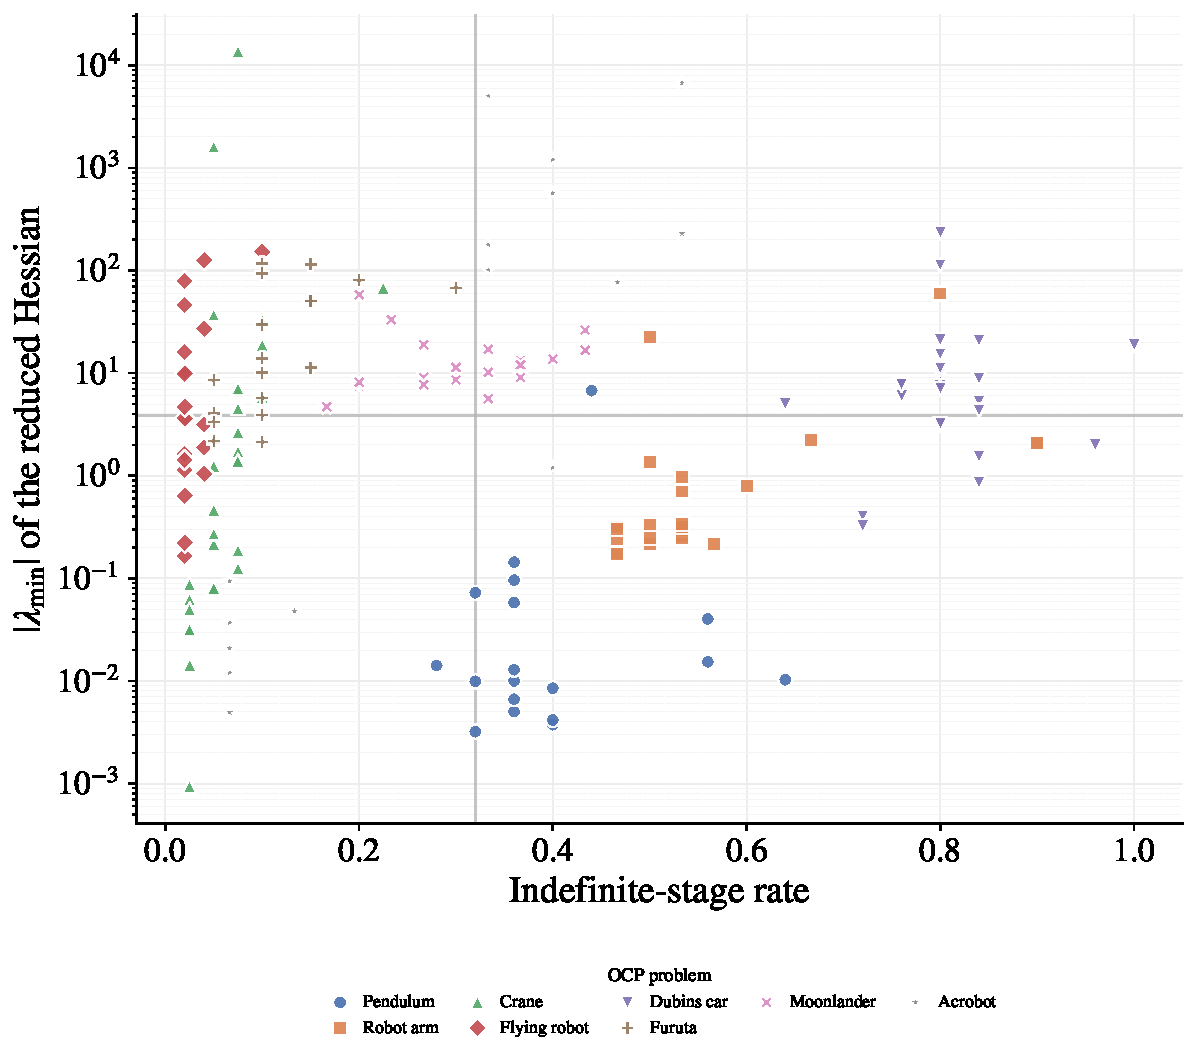
\includegraphics[width=0.95\textwidth]{images/benchmark/indefiniteness_coverage_scatter.pdf}
    \caption{Depth ($|\lambda_{\min}|$ of the reduced Hessian, log scale)
    versus width (indefinite-stage rate) of the collected QPs, coloured by
    OCP problem.}
    \label{fig:indefinite_qp_scatter}
\end{figure}

As seen from Figure~\ref{fig:indefinite_qp_scatter}, the collected indefinite QPs do not concentrate in a single regime.
They spread over more than seven orders of magnitude in depth ($|\lambda_{\min}|$ ranging from about $10^{-3}$ to $10^{4}$).
And the coverage is strongly problem-dependent: each OCP occupies a characteristic region of the depth--width plane rather than scattering uniformly.

Two complementary major patterns can be observed.
Problems that are indefinite in only a small fraction of their stages, such as \texttt{overhead\_crane},
\texttt{free\_flying\_robot} and \texttt{furuta\_cons}, nevertheless reach very deep negative curvature:
their indefinite-stage rates stay below $0.30$ (with medians of $0.05$, $0.02$ and $0.10$, respectively),
while $|\lambda_{\min}|$ reaches up to $10^{2}$--$10^{4}$.
Conversely, problems with a high indefinite-stage rate, \texttt{dubins\_car\_parallel\_parking} and \texttt{robot},
with rates ranging from $0.47$--$1.0$, tend to exhibit only moderate depth,
with $|\lambda_{\min}|$ clustered around $10^{-1}$--$10^{1}$.
Broad and deep indefiniteness thus appear to occur largely separately rather than together.

Some problems also fall in the middle, such as \texttt{moonlander} and
\texttt{acrobot}, which occupy intermediate indefinite-stage rates
(roughly $0.07$--$0.53$). \texttt{moonlander} keeps its depth in a narrow band
($|\lambda_{\min}|$ between $10^{0}$ and $10^{2}$), whereas \texttt{acrobot}
scatters over almost the entire depth range, from near-singular values around
$10^{-2}$ up to nearly $10^{4}$. They neither confine their negative curvature
to a few stages nor spread it across the whole horizon, and thus bridge the two
extreme regimes rather than belonging clearly to either.

Taken together, the eight OCPs cover a broad range of the depth--width plane:
from narrow-but-deep (\texttt{overhead\_crane}, \texttt{free\_flying\_robot}, \texttt{furuta\_cons}),
through intermediate (\texttt{moonlander}, \texttt{acrobot}),
to broad-but-moderate (\texttt{dubins\_car\_parallel\_parking}, \texttt{robot}),
with \texttt{pendulum\_cons} adding cases of very shallow negative curvature
($|\lambda_{\min}|$ mostly below $10^{-1}$) at intermediate indefinite-stage rates.
This spread indicates that the collected QP subproblems exercise indefiniteness across qualitatively different regimes rather than a single one.

\begin{figure}[H]
    \centering
    \begin{minipage}[t]{0.48\textwidth}
        \centering
        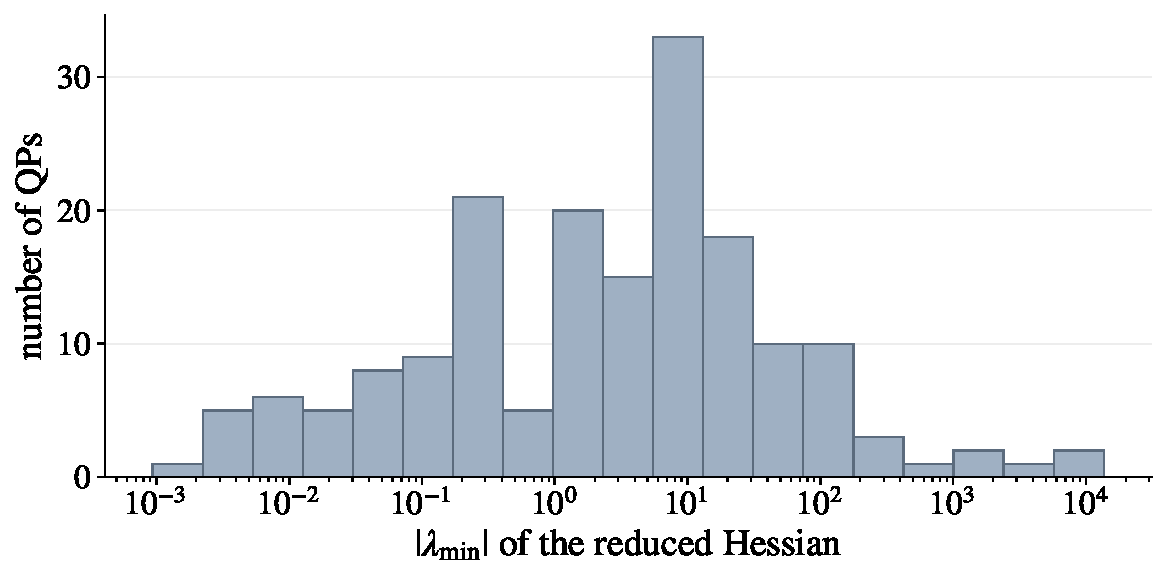
\includegraphics[width=\linewidth]{images/benchmark/indefiniteness_coverage_depth.pdf}
        \subcaption{Depth: distribution of $|\lambda_{\min}|$.}
        \label{fig:indefinite_depth}
    \end{minipage}
    \hfill
    \begin{minipage}[t]{0.48\textwidth}
        \centering
        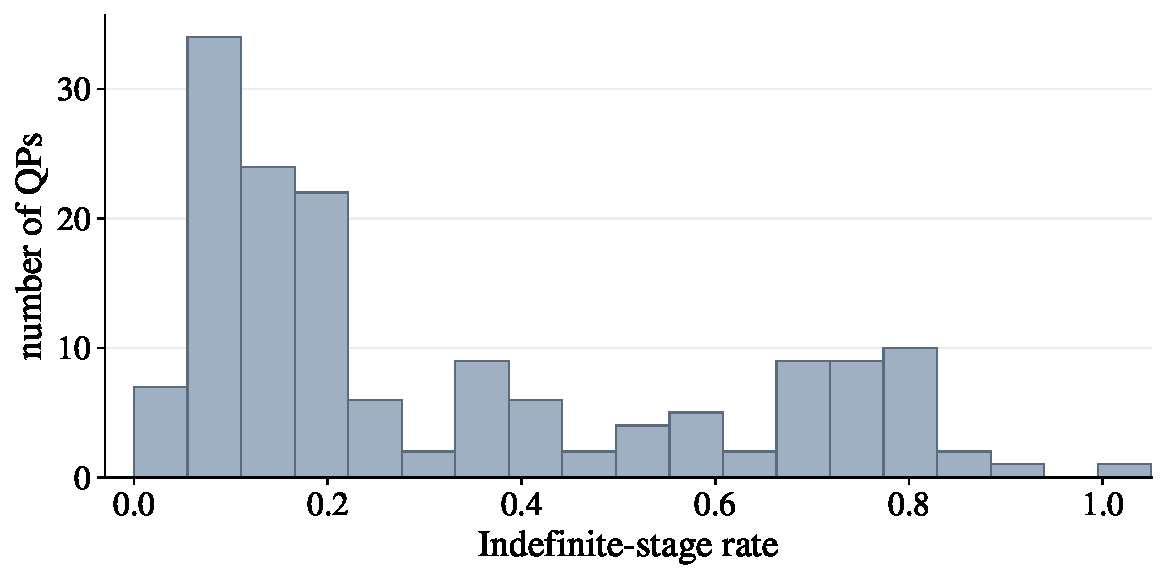
\includegraphics[width=\linewidth]{images/benchmark/indefiniteness_coverage_breadth.pdf}
        \subcaption{Width: distribution of the indefinite-stage rate.}
        \label{fig:indefinite_breadth}
    \end{minipage}
    \caption{Marginal distributions of depth and width over all collected QPs.}
    \label{fig:indefinite_marginals}
\end{figure}

Figure~\ref{fig:indefinite_marginals} shows the two marginal distributions of the same data. The depth histogram
(Figure~\ref{fig:indefinite_depth}) is centred around $|\lambda_{\min}| \approx 10$, where most of the indefinite QPs lie,
with roughly one third of all instances falling between $10^{0.5}$ and $10^{1.5}$,
and decays toward both a near-singular tail near $10^{-3}$ and a small number of very deep cases at $10^{3}$--$10^{4}$,
of which only five instances exceed $10^{3}$.
Hence, although extreme cases exist, the negative curvature typically encountered during the SQP iterations is of moderate magnitude.

The width histogram (Figure~\ref{fig:indefinite_breadth}) shows how the indefinite-stage rate is distributed over the collected QPs. The rate
covers the full range up to~$1$, with a large share of QPs being indefinite in only a minority of their stages:
close to $40\%$ of the instances have a rate below $0.11$. The remainder is spread out
with a secondary accumulation around rates of $0.33$--$0.55$ and a further group around $0.72$--$0.88$,
while only a single QP is indefinite in essentially all of its stages.

This is consistent with the scatter plot: for most problems only a subset of stages become indefinite, whereas a few problems
(\texttt{dubins\_car\_parallel\_parking}, \texttt{robot}) are indefinite across the majority of their stages.

\subsection{Source of Indefiniteness}
\label{subsec:source}
Recalling the block reduced Hessian at $k$ stage is calculated as $M_k = R_k + B^\top P_{k+1}B$,
which is assembled from two contributions: the control cost block $R$ and the cost-to-go block $P$. 

To understand \emph{where} the indefiniteness originates,
we classify every indefinite stage according to which of the two blocks has a negative smallest eigenvalue: 
\emph{R only} ($R$ indefinite, $P$ definite), \emph{P only} ($P$ indefinite, $R$ definite), and \emph{both} (both indefinite).

\begin{figure}[H]
    \centering
    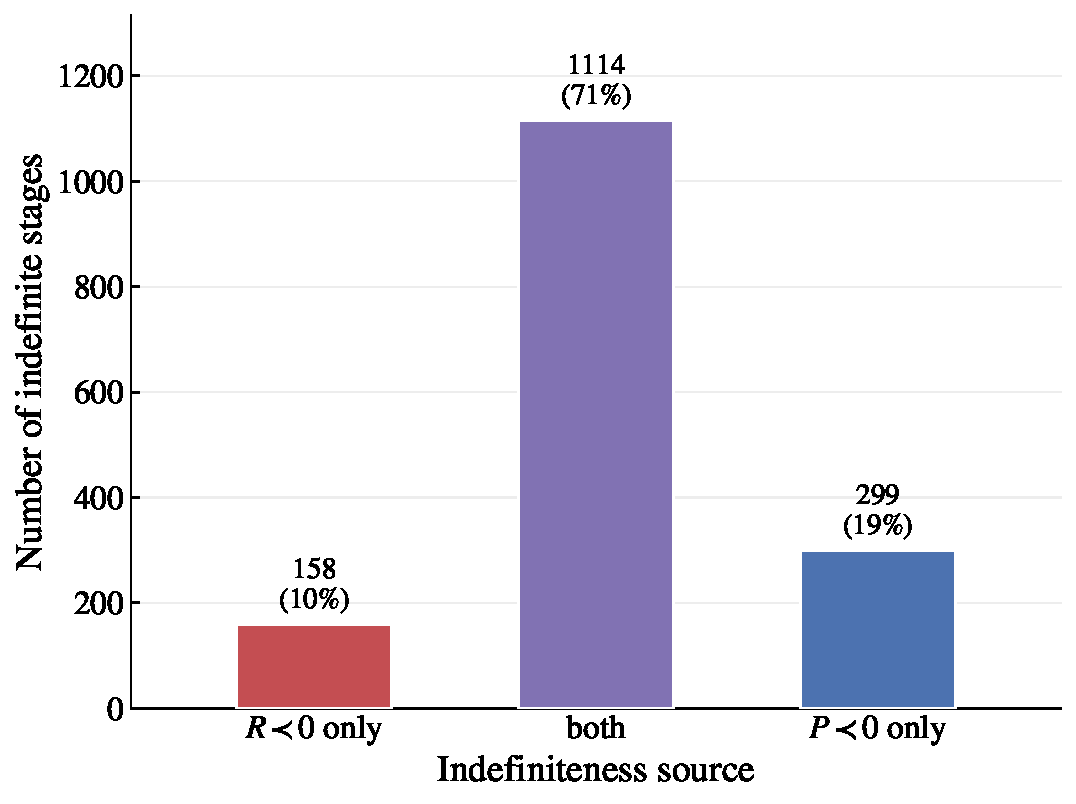
\includegraphics[width=0.7\textwidth]{images/benchmark/stage_indefiniteness_source.pdf}
    \caption{Number of indefinite stages by source: control cost~$R$,
    cost-to-go~$P$, or both.}
    \label{fig:indefinite_source_counts}
\end{figure}

Figure~\ref{fig:indefinite_source_counts} aggregates all indefinite stages across the benchmark. 
The dominant source is the joint case: $1114$ of the $1571$ indefinite stages ($71\%$) have \emph{both} $R$ and $P$ indefinite, 
so in the large majority of cases the negative curvature is not confined to a single block. 
Among the remaining stages where only one block is indefinite, 
the cost-to-go block is the more frequent culprit: $P$ alone accounts for $299$ stages ($19\%$), 
nearly twice the $158$ stages ($10\%$) in which only the control cost $R$ is indefinite. 

Overall, the cost-to-go block $P$ is indefinite more often than the control cost block $R$,
being involved in $1413$ of the $1571$ indefinite stages ($90\%$) against $1272$ ($81\%$) for $R$,
which indicates that the indefiniteness is driven primarily by the cost-to-go term rather than by the control cost.

\begin{figure}[H]
    \centering
    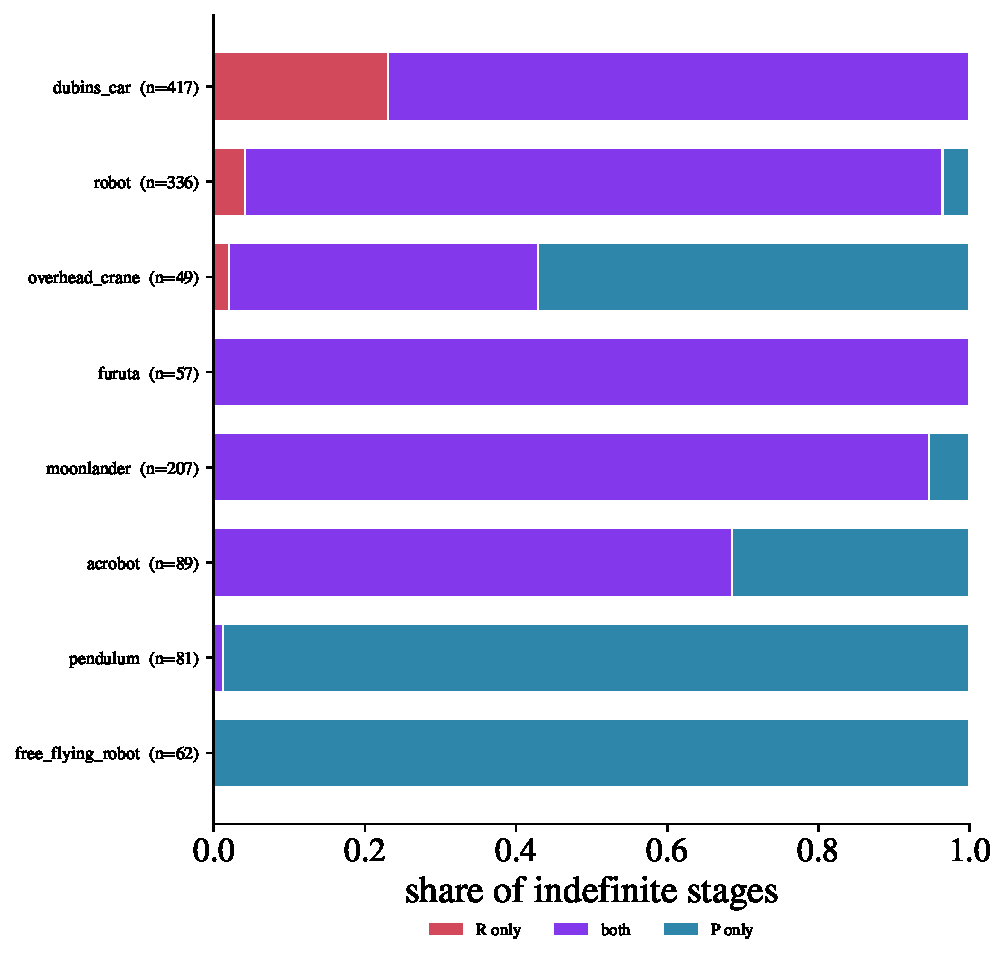
\includegraphics[width=1.0\textwidth]{images/benchmark/stage_indefiniteness_signature.pdf}
    \caption{Per-problem composition of stage indefiniteness. Each bar
    shows, for one OCP, the share of stages that are \emph{R only},
    \emph{both}, \emph{P only}, ($n$ is the number of collected indefinite stages).}
    \label{fig:indefinite_source_signature}
\end{figure}

While Figure~\ref{fig:indefinite_source_counts} gives the aggregate picture,
Figure~\ref{fig:indefinite_source_signature} breaks the same classification down per problem and reveals a strongly problem-dependent and clean structure: 
six of the eight OCPs are dominated by a single category ($\geq\!70\%$ of their stages),
three of them almost exclusively so ($\geq\!90\%$),
and only \texttt{acrobot} and \texttt{overhead\_crane} are genuinely mixed.

As observed from Figure~\ref{fig:indefinite_source_signature},
most of the problems are governed by the \emph{both} case, 
including \texttt{moonlander} ($96\%$), \texttt{robot} ($92\%$), \texttt{dubins\_car\_parallel\_parking} ($76\%$)
and \texttt{furuta\_cons} ($72\%$).
Notably, three problems (\texttt{dubins\_car\_parallel\_parking}($n=581$), \texttt{robot}($n=404$) and \texttt{moonlander}($n=198$)), contribute by far the most indefinite stages, 
they largely account for the aggregate dominance of the \emph{both} case reported above. 

The \emph{P only} case dominates the remaining problems: \texttt{free\_flying\_robot} is indefinite purely through the cost-to-go block ($100\%$),
and \texttt{pendulum\_cons} nearly so ($87\%$). The two mixed problems lean the same way:
\texttt{overhead\_crane} splits into $58\%$ \emph{P only} against $39\%$ \emph{both},
and \texttt{acrobot} into $54\%$ \emph{P only} against $41\%$ \emph{both},
so that even where no single category dominates, the cost-to-go block is the more frequent one.
Taken over all stages, the cost-to-go block is indefinite in the large majority of cases, 
whereas the \emph{R only} case is marginal:
it appears in only four problems and is negligible for \texttt{robot}, \texttt{acrobot} and \texttt{overhead\_crane} (all below $5\%$), 
with \texttt{dubins\_car\_parallel\_parking} being the sole problem where isolated $R$-block indefiniteness is substantial ($24\%$ of its stages,
accounting for $140$ of the $158$ \emph{R only} stages in the whole benchmark). 
Indefiniteness therefore predominantly involves the cost-to-go block, 
either alone or jointly with $R$, while $R$-block-only indefiniteness is the exception.

In conclusion, these figures numerically shows that,
across the benchmark the cost-to-go block is involved in the vast majority of indefinite stages, 
a regularization strategy that merely enforces $M\succ 0$ would therefore leave the negative curvature unaddressed in most stages. 
Since the cost-to-go term enters the reduced Hessian through $M_k = R_k + B^\top P_{k+1} B$, 
keeping $P_{k+1}$ (and hence $M_k$) definite is essential for a reliable regularization method, 
whereas treating the control cost block alone is not sufficient.

\end{document}
    \documentclass[class=scrbook, crop=false]{standalone}
\usepackage[subpreambles=true]{standalone}
\ifstandalone
    \input{../settings+/settings}
\fi

% ----------------------------------------------------------------------------
%                               Results
% ----------------------------------------------------------------------------
\begin{document}

\chapter{Numerical Experiments} % Overview text


\section{Iteration Profile and Flop Units Estimation}

\section{Experiment Setup}

    \subsection{Prototype Solver Implementation}
    We implemented a Riccati-based IPM solver in python, which produces similar iteration behavior as HPIPM in convex QPs with certain solver settings.
    It is basically just HPIPM in detla formulation without iterative refinement, the setting is as following:
    
    TODO: have a setting table for explaining this.
 
    We test the solver with convex QP subproblems from the OCPs in benchmark, the iteration profile is as follows:

    TODO: Insert the fig

    \subsection{General setup}
    With the Python prototype, we further implement the following regularizations in the solver as:
    \begin{itemize}
        \item PROJECT
        \item MIRROR
        \item PRECOMPUTE
        \item PM\_STAGE\_MIRROR
        \item PM\_STAGE\_GMW
        \item INERTIA\_CORRECTION
    \end{itemize}


\section{Numerical Results}
    \subsection{Mehrotra's Predictor-Corrector with Funnel Line Search}
    \subsection{Mehrotra's Probing with Funnel Line Search}
    \subsection{Mehrotra's Probing without Funnel Line Search}


\section{Possible Disscusion}

\end{document}

    \documentclass[class=scrbook, crop=false]{standalone}
\usepackage[subpreambles=true]{standalone}
\ifstandalone
    \input{../settings+/settings}
\fi

% ----------------------------------------------------------------------------
%                               Conclusion
% ----------------------------------------------------------------------------
\begin{document}

\chapter{Conclusion and Outlook} % Overview text
\label{Chapter::Conclusion}

This thesis regularized the indefinite QPs that arise in exact-Hessian SQP for NMPC at the QP level, inside the interior point solver,
where the barrier curvature is already taken into account and only the reduced Hessian needs to be positive definite.
We showed that the Riccati backward pass is a block $\mathrm{LD}\mathrm{L}^\top$ factorization of the reduced Hessian,
so that indefiniteness is detected and corrected stage-wise wherever the Cholesky factorization of $\tilde{M}_k$ fails,
while the linear complexity of the recursion in the horizon length is preserved.
We further showed that the minimum-perturbation rule propagates negative curvature through the cost-to-go matrix to the preceding stages.
This led to an improved strategy that uses a non-minimal correction and also regularizes the cost-to-go matrix,
and we proved that the regularization becomes inactive close to the solution, so that the local convergence rate of the interior point method is retained.

On a benchmark of $175$ indefinite QPs from eight OCPs,
whose analysis showed that the cost-to-go matrix is involved in most indefinite stages,
\textsf{PM\_MIRROR} left $4$ instances unsolved and \textsf{PM\_GMW} $7$ at a lower cost,
against $32$ to $59$ for full Hessian regularization and $15$ for inertia correction.
The full Hessian methods failed on almost every \textsl{Flying robot} instance, where the indefiniteness is confined to the cost-to-go matrix at a few stages,
and the instances left unsolved by all methods combine deep negative curvature with a large share of indefinite stages.

Several questions remain open:
\begin{itemize}
    \item \textbf{Regularization magnitude.} The eigenvalue floor $\epsilon$ is fixed,
    and the remaining failures occur where large corrections are applied at many stages.
    Adapting the magnitude, e.g.\ to the conditioning of the corrected blocks or to the barrier parameter, could improve robustness.
    \item \textbf{Other MPC formulations.} In time-optimal and economic MPC,
    the cost provides little positive curvature, so indefiniteness is likely to be broader than in this benchmark.
    Whether the ranking of the methods carries over remains to be tested.
    \item \textbf{Embedding in SQP.} The QPs were solved in isolation with a Python prototype.
    An implementation in HPIPM and \texttt{acados} is needed to compare against SQP-level regularization
    in terms of SQP iterations, run time and closed-loop performance.
\end{itemize}

\end{document}

    \include{chapters/acknowledgments}

    % Bibliography
    \printbibliography[heading=bibintoc]                            \cleardoublepage

    % -------------------------------------------------------------------------------
    % Appendix and Glossary
    % -------------------------------------------------------------------------------
    \pagenumbering{Alph} % A, B, C..

    % Appendix
    \include{chapters/appendix}

    % print main glossary
    %       type=main           glossary
    %       type=symbolslist    list of symbols
    %       type=acronyms       list of acrononyms
    \printglossary[type=main]

    % Either print all entries or only used entries for all lists
    % \glsaddallunused

\end{document}